\documentclass[11pt,a4paper,twoside]{report}

%--------------------------------------------------
% global definitions to be used in the front page
%--------------------------------------------------
\providecommand{\coursename}{Design and Implementation of Mobile Applications}
\providecommand{\documentsubtitle}{Design Document}
\providecommand{\annoacc}{2012-2013}
\providecommand{\principaladviser}{Prof. Luciano Baresi}
\providecommand{\firstauthor}{Claudio Rizzo}
\providecommand{\firstauthorid}{800471}
\providecommand{\secondauthor}{Emanuele Uliana}
\providecommand{\secondauthorid}{799256}

\title{Watch Dog}
\author{\firstauthor, \secondauthor}

\usepackage[margin=3cm]{geometry} % margins set here are for the TITLE page...


\usepackage[utf8]{inputenc}
\usepackage[english]{babel}
\usepackage{tikz}
\usetikzlibrary{arrows,positioning, decorations.text}

\usepackage{graphicx}
\usepackage{booktabs}
\usepackage{listings}

\lstset{columns=fullflexible}

\usepackage[T1]{fontenc}
\usepackage{palatino}
\usepackage{mathpazo} 
\lstset{basicstyle=\ttfamily}

\usepackage[pdfauthor={\firstauthor, \secondauthor}, pdftitle={WatchDog - Design Document}, colorlinks, linkcolor=black, urlcolor=black]{hyperref}

\usepackage{amsmath}
\usepackage{amsthm}
\newtheoremstyle{note} % name
	{\topsep} 	% Space above
	{\topsep} 	% Space below
	{\small}		% Body font
	{}		% Indent amount
	{\small\bfseries}% Theorem head font
	{:}		% Punctuation after theorem head
	{.5em}	% Space after theorem head
	{}		% Theorem head spec (can be left empty, meaning ‘normal’)
\theoremstyle{note}
\newtheorem*{nota}{Nota}	
%
\usepackage{settings/frontesp}




\usepackage{fancyhdr}
%% Cambia il carattere delle didascalie delle figure %%
\usepackage[font=small,format=plain,labelfont=bf,up,textfont=it,up]{caption}


%per le tabelle lunghe e particolari
\usepackage{lscape}

\setlength{\parindent}{0in}  %%solo una proposta: così non serve
% più il \noindent dopo \\

%% Alloy code begins
\usepackage{color}
\usepackage{xcolor}
\usepackage[normalem]{ulem}
\usepackage{caption}
\DeclareCaptionFont{white}{\color{white}}



%%%%% 

%e.g.
%\begin{lstlisting}[label=some-code,caption=Some Code]
%public void here() {
%	goes().the().code()
%}
%\end{lstlisting}



%Alloy code ends





\begin{document}


\titlep
\newgeometry{top=4cm,bottom=4cm,right=4cm,left=4cm}
%% STILE DELLE INTESTAZIONI %%

\pagestyle{fancy}
\renewcommand{\chaptermark}[1]{\markboth{#1}{}} % aggiungi \thechapter.\ per anche il numero capitolo
%\renewcommand{\sectionmark}[1]{\markright{#1}} % titoli di sezione
\fancyhf{}
\fancyhead[RE,RO]{\small\thepage}
\fancyhead[LE,LO]{\small\em\leftmark} % \leftmark = 2.TitoloCapitolo, \rightmark = TitoloSezione
%\fancyhead[LO]{\small\em\rightmark}  % LO = Left Odd, RO = Right Odd, LE = Left Even, RE = Right Even
\fancypagestyle{plain}{ % titolo di sezione e simili
	\fancyhf{} % remove everything
	\renewcommand{\headrulewidth}{0pt} % remove lines as well
	\renewcommand{\footrulewidth}{0pt}
}

%%% Cambia il carattere dei titoli di sezione %%
%\usepackage{titlesec}
%\titleformat{\section}{\Large\bfseries\sffamily}{\thesection}{1em}{}

%% Stile dei titoli di capitolo %%
\makeatletter
\def\thickhrulefill{\leavevmode \leaders \hrule height 0.7ex \hfill \kern \z@}
\def\@makechapterhead#1{%
  \vspace*{10\p@}%
  {\parindent \z@ \centering \reset@font
        %\thickhrulefill
        \par\nobreak \vspace{3\p@}
        {\huge \bfseries \rmfamily \strut \thechapter.\ #1}\par\nobreak
        \interlinepenalty\@M
        \hrule
        \vspace*{10\p@}%
    \vskip 30\p@
  }}

\def\@makeschapterhead#1{%
  \vspace*{10\p@}%
  \vspace*{10\p@}%
  {\parindent \z@ \centering \reset@font
        %\thickhrulefill
        \par\nobreak \vspace{3\p@}
        {\huge \bfseries \rmfamily \strut #1}\par\nobreak
        \interlinepenalty\@M
        \hrule
        \vspace*{10\p@}%
    \vskip 30\p@
  }}

\tableofcontents
\cleardoublepage


% --------------------------------------------------------------------------------------------------------------------
% Capitoli

% \include con i nomi dei capitoli

\chapter{Project context and purpose }
\label{cap:Introduction} 

\section{Context}

Watchdog is an application for Android devices developed by Claudio Rizzo
and Emanuele Uliana for the "Design and Implementation of Mobile Appli-
cations" (DIMA in short) course at "Politecnico di Milano, Corso di studi in
Ingegneria Informatica Magistrale". The advisor is professor Luciano Baresi
from the Deepse (Dependable, Evolvable, Pervasive Software Engineering)
group of the Deib (Dipartimento di Elettronica, Informazione e Bioingegne-
ria).

\section{Purpose}

The application purpose is to provide a way to remote control a mobile phone
from another cellphone: this is very useful in case of theft or loss, since it’s
possible to localize the target phone or to trigger a full volume repeating
alarm sound. The application is mainly intended to be used by the same user
on two (or more) different mobiles, althought it’s not mandatory.



\chapter{Project Planning}
\label{cap:Planning} 

\section{Overview}

We had the idea to develop a remote control application after seeing there
was not something similar not embedded in a more general application (in
fact every anti-malware for mobile devices have a similar functionality, but it
comes along with many others features) and because we really like the se-
curity/privacy (and cryptography) aspects of computer science. We planned
the security/cryptography aspects from the beginning, such that the Confi-
dentiality/Integrity/Availability paradigm is always respected along with the
extremely important authentication and non-repudiation aspects.

\chapter{Requirements Analysis}
\label{cap:RequirementsAnalysis} 


\section{Actors}

As said before, the main actor is usually a single user which uses the ap-
plication on two different mobile phones, one being the stolen/lost one and
the other the rescue one. It’s also possible a second actor to exists: a (very)
trusted friend may be the one who sends remote commands to the target tele-
phone; since a password authentication scheme is employed, it’s not possible
to do any abuse in this case.

\section{Functional Requirements}

The application allows the user do to the following tasks:

\begin{itemize}
 \item Initialization
 \item Mobile Phone Association
 \item Password Change
 \item Unilateral Deassociation
 \item Remote Localization
 \item Mobile Phone Mark
 \item Remote Alarm Triggering
 \item Local Alarm Off
 \item Perimeter Selection
\end{itemize}

\section{Non Functional Requirements}

The remote control of a cellphone is a critical activity and has many security
and privacy requirements: the next paragraphs show them briefly: for in-depth
explainations see the design section (4.3). %metti il riferimento latexiano

\subsection{Privacy and Security: problems and Solutions}

\bfseries 
Sender authentication:
\normalfont
While the sender (telephone) authentication plays indeed a key role, it’s even
more crucial the authentication of the person behind a control message; that’s
the reason for employing a password based authentication scheme: in the
initialization wizard the user is required to insert a password which is going
to be needed to send a message to that telephone (the basic assumption
is the password is known only by the mobile owner and by some people,
possibly no one, he trusts). The password is stored hashed with SHA-256 in
the application preferences, along with the hashing salt (a random token) to
avoid both time-to-memory attacks (such as rainbow tables) and the equality
of two hashes generated from two equal passwords; the salt is sent to another
telephone after the process of public keys authentication (See section 4.3.6).


\bfseries 
Integrity:
\normalfont
The message received must be exactly the one sent: every transmission error
or tampering must be detected and cause the abort of the current command
session: no retransmission is done.


\bfseries
Authentication:
\normalfont
The receiver must have a secure way to understand which telephone the
received message comes from.


\bfseries 
Non forgeability:
\normalfont
Nobody should be able to forge a command message which is both valid and
correctly authenticated.


\bfseries 
Non Repudation:
\normalfont
The sender must not be able to deny he sent a specific message (if he actually
did it).
Digitally signing every command message can ensure integrity, authentica-
tion, non repudiation and a weak defense against non forgeability: symmetric
encryption (and in particular AES-256 in GCM mode of operation) is needed
for full protection.


\bfseries
Message Confidentiality:
\normalfont
No one should be able to detect that and which command is sent to a mobile
phone, so the command message is encrypted with the symmetric cipher
AES-256 in GCM mode of operation (used for performance reasons and for a
supplementary integrity check).



\bfseries
Asymmetric keys management:
\normalfont
Asymmetric keys management
Digital signatures (and shared secrets computation as we will see) require
asymmetric cryptography: in the initialization wizard the application gener-
ates and stores in the preferences a key pair based on the elliptic curves; the
reasons for this choice are performances and the smaller key length with re-
spect to other keys (like RSA and DSA ones) at a fixed level of security. This
makes the 140 characters (bytes) Android limit for a single sms no more a
problem.


\bfseries
Symmetric key/initialization vector management:
\normalfont
AES-256, being a symmetric cipher, encrypts and decrypts a specific message
with the same key, and, given the communication channel is not secure, the
two parts must agree on the same key in some way; in particular ECDH is
used to compute a common secret once and for all, then, when in need to
send a message, the sender picks up a random 32 bytes salt, forwards it to
the receiver, then both parts use a keyschedule algorithm (PBKDF2 with
HMAC-SHA-256) to derive the same key starting from the secret and the
salt. Furthermore the GCM mode of operation requires for every message the
sender to generate a 12 bytes random initialization vector and to send it to
the receiver.


\bfseries
Public keys mutual authentication:
\normalfont

While dealing with asymmetric cryptography, the main problem is to bind a
public key with a real user to avoid active Man-In-The-Middle (MITM from
now on) attacks. Neither a Pulic Key infrastructure (PKI) or a Web Of Trust
(WOT) is employed, because they are both potentially insecure for various
reasons (in the PKI case the presence of a trusted element, a certification
autorithy hierarchy, which may be compromised/untrusted/fake; in the WOT
case the presence of a net of trusted elements, the ones who signed a specific
public key, which might be fake/bad persons; furthermore a key with no
signatures is not automatically a fake one, but there isn’t a way to tell), so
the application uses a modified version of the Socialist Millionaire Protocol
(SMP) to authenticate to each one each other key; this requires the two parts
to have a common secret (an answer to a particular question set up on the fly
by the users during the SMP), which is easy to achieve, since the two users
are likely to be the same person or two people who trust themselves.

\subsection{Performance}

We chose the crypto algorithms with an eye on the performances of the
whole system: the key idea is the bottleneck must be the sms and not the
computation time required by the encryptions/decryptions; for this reason
the command messages are encrypted with a symmetric algorithm and not
with RSA or ElGamal (or another asymmetric algorithm), since symmetric
cryptography is faster than asymmetric at least by two orders of magnitude
(they are very likely to be 3 anyway); however to do ECDH and ECDSA
the application needs also an asymmetric key pair, which is generate during
the intitial wizard once an for all, so an acceptable overhead. The public
keys mutual validation (SMP + ECDH in practice) takes some time, but it’s
done only one time per association, which means two telephones have to do it
only when they associate themselves. Finally the digital signature/verification
process are quite fast and so is the key-derivation from the secret and the
salt.











\chapter{Use Cases}
\label{cap:UseCases} 


\section{Initialization}
The first time the appliction is opened the user sees a welcome message and his
prompted to comlete the initialization wizard which consists in selecting and
confirming a password which will be the one needed by other telephones/users
to send commands to that mobile. The password scheme forces to select an
alphanumeric string (some special characters are also allowed) between 8-
20 characters and with at least a letter and a number. In case of error
(bad password/confirmation password different from the base one) the user is
notified back and asked to retry. In case of success the application redirects
to the main view, which is the "sms localization" one.

\subsection{Activity Diagram}

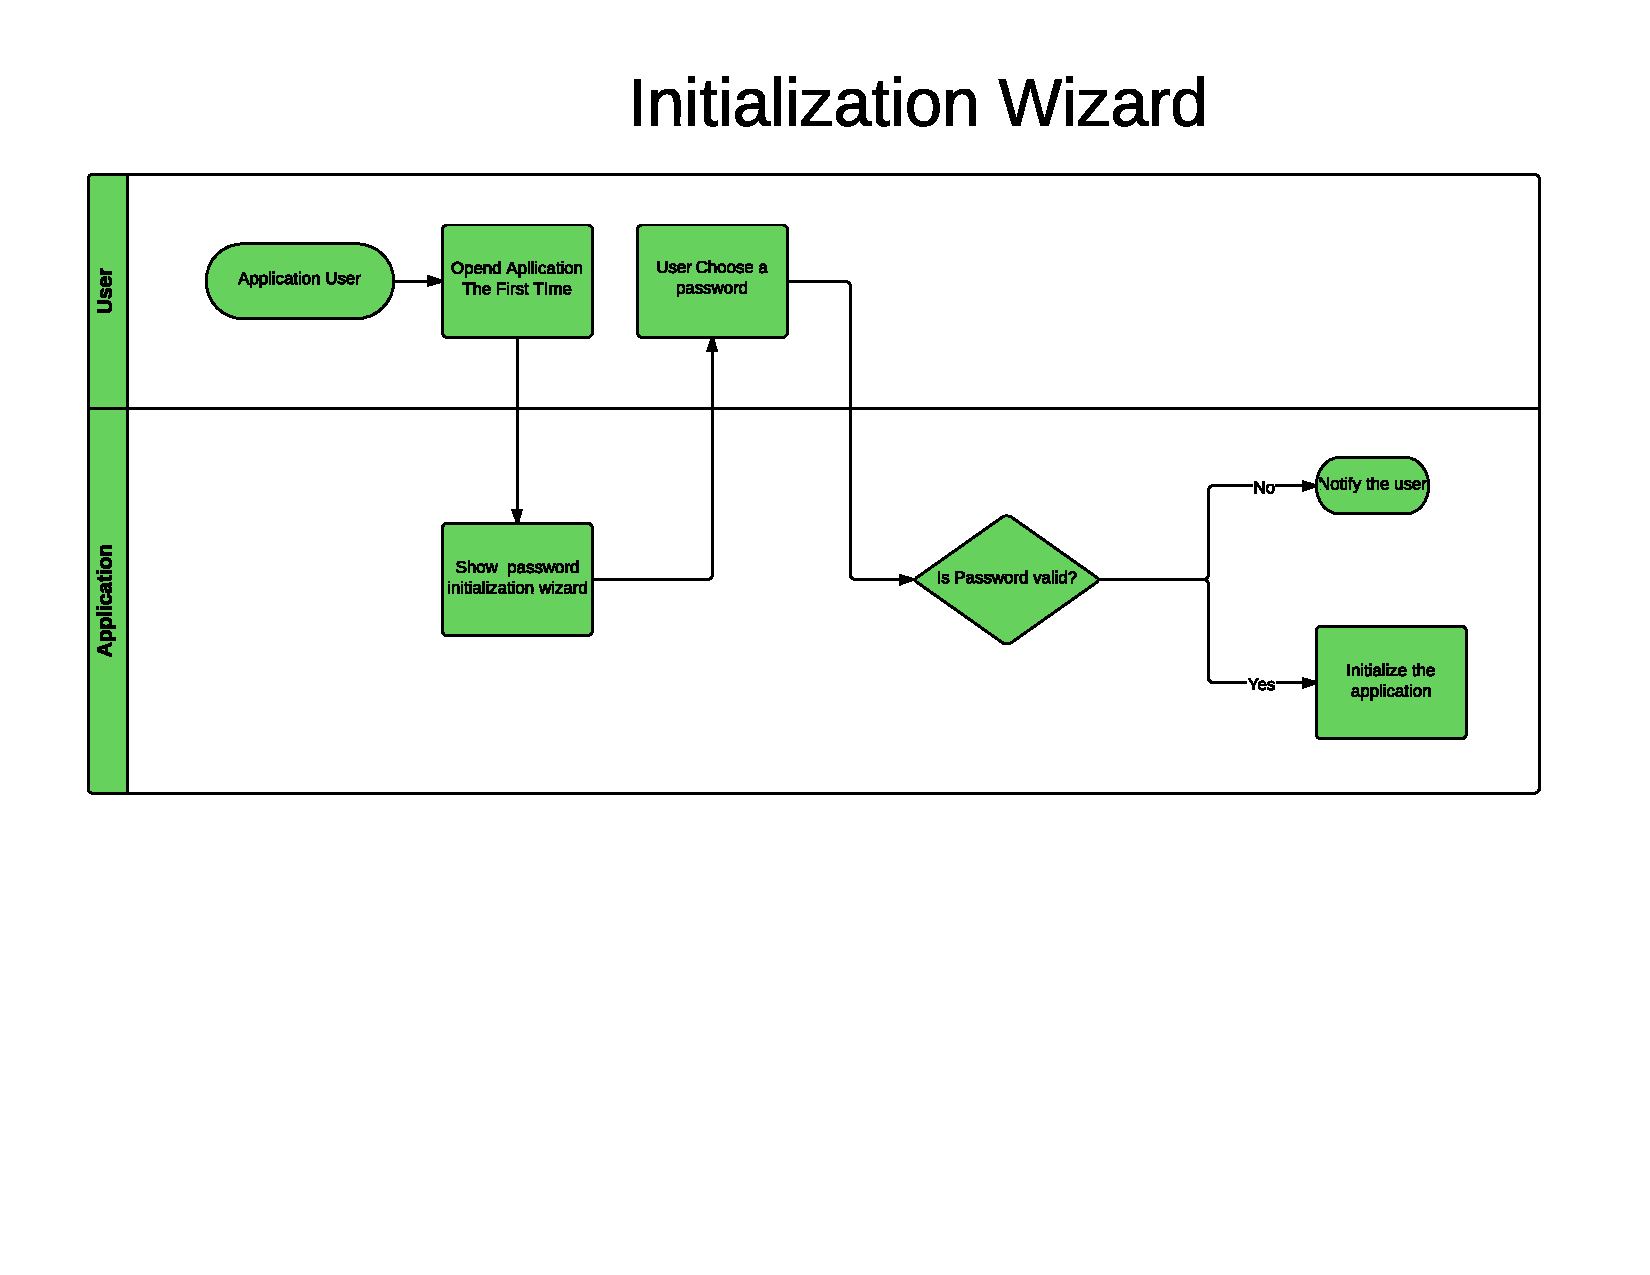
\includegraphics[scale=0.5]{images/initialization_activity}

\newpage
\subsection{User Interface Design}

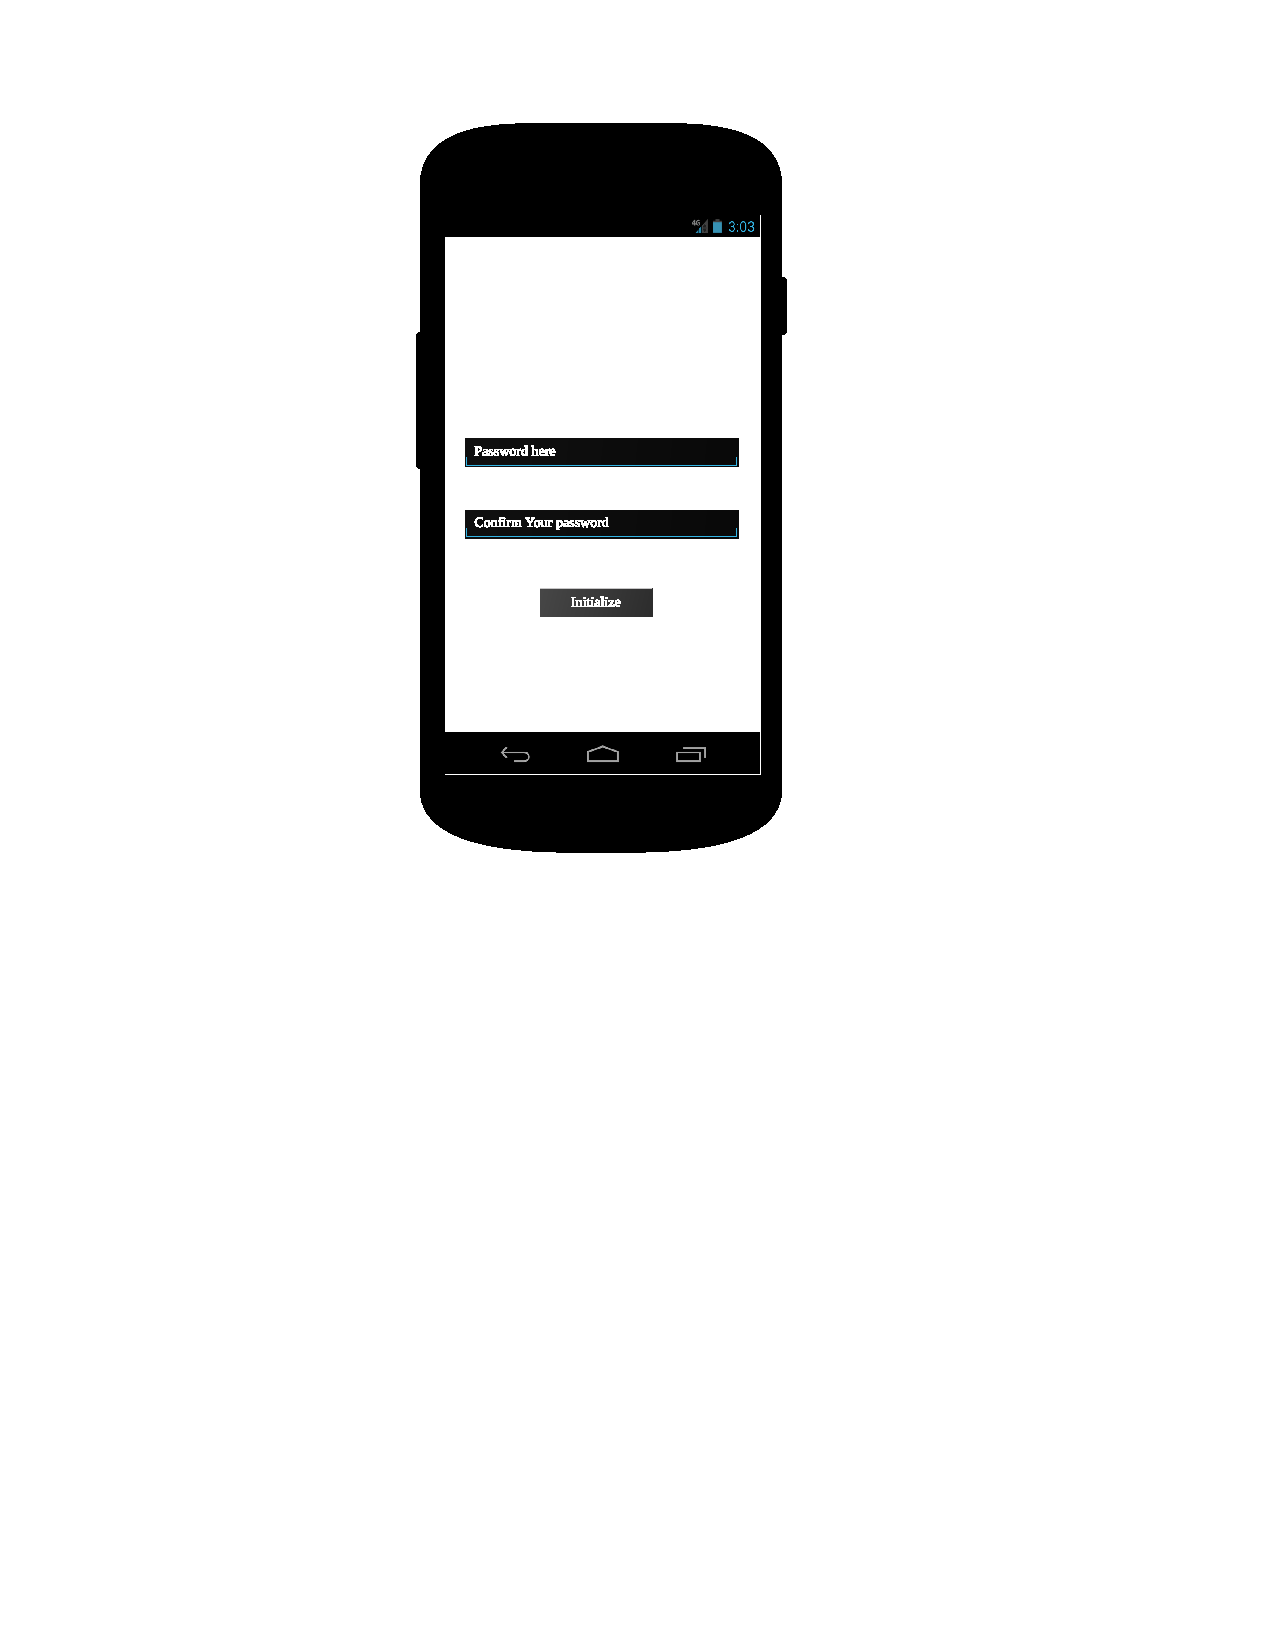
\includegraphics[scale=0.7]{images/initialization_design}


\section{Mobile Phone Association}
For enhanced security it’s required two telephones are associated before they
can send commands to the other one; the association is bidirectional and can
be removed only locally (the other telephone won’t know anything, but will
obviously fail in sending commands). This totally cuts away the possibility of
a Man In The Middle (MITM) both active and passive. A user who wants
to associate his telephone with another one first selects a secret question
and a secret answer and sends the first to the other mobile, whose user can
decide to accept or refuse the request. In the second case the first user is
notified back and the association ends with a "failure", otherwise the second
user types what he thinks is the secret answer and selects his own secret
question/answer. The first user now has to type the answer to that question
and, if all goes smooth, the association is done. Every passage is done by
sms sending.

\newpage
\subsection{Activity Diagram}

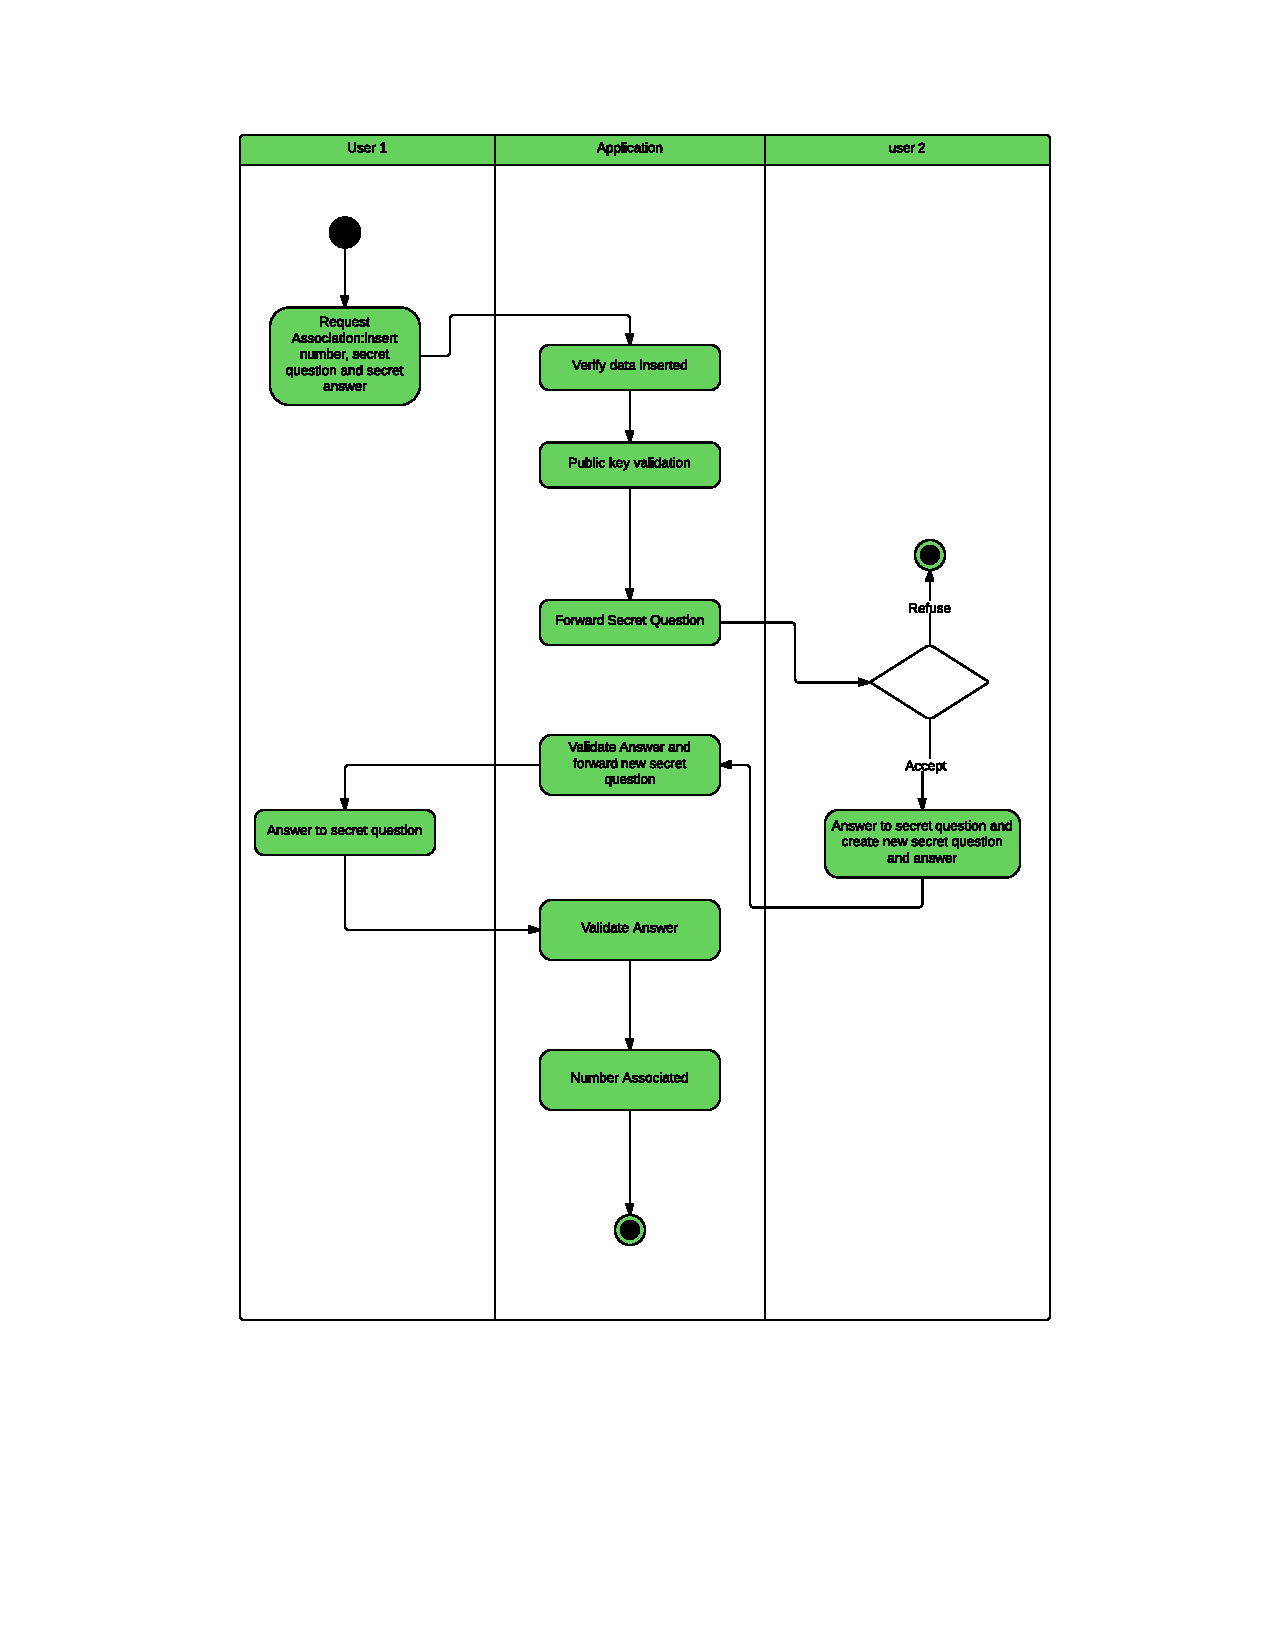
\includegraphics[scale=0.7]{images/SMP_activity}

\newpage
\subsection{User Interface Design}

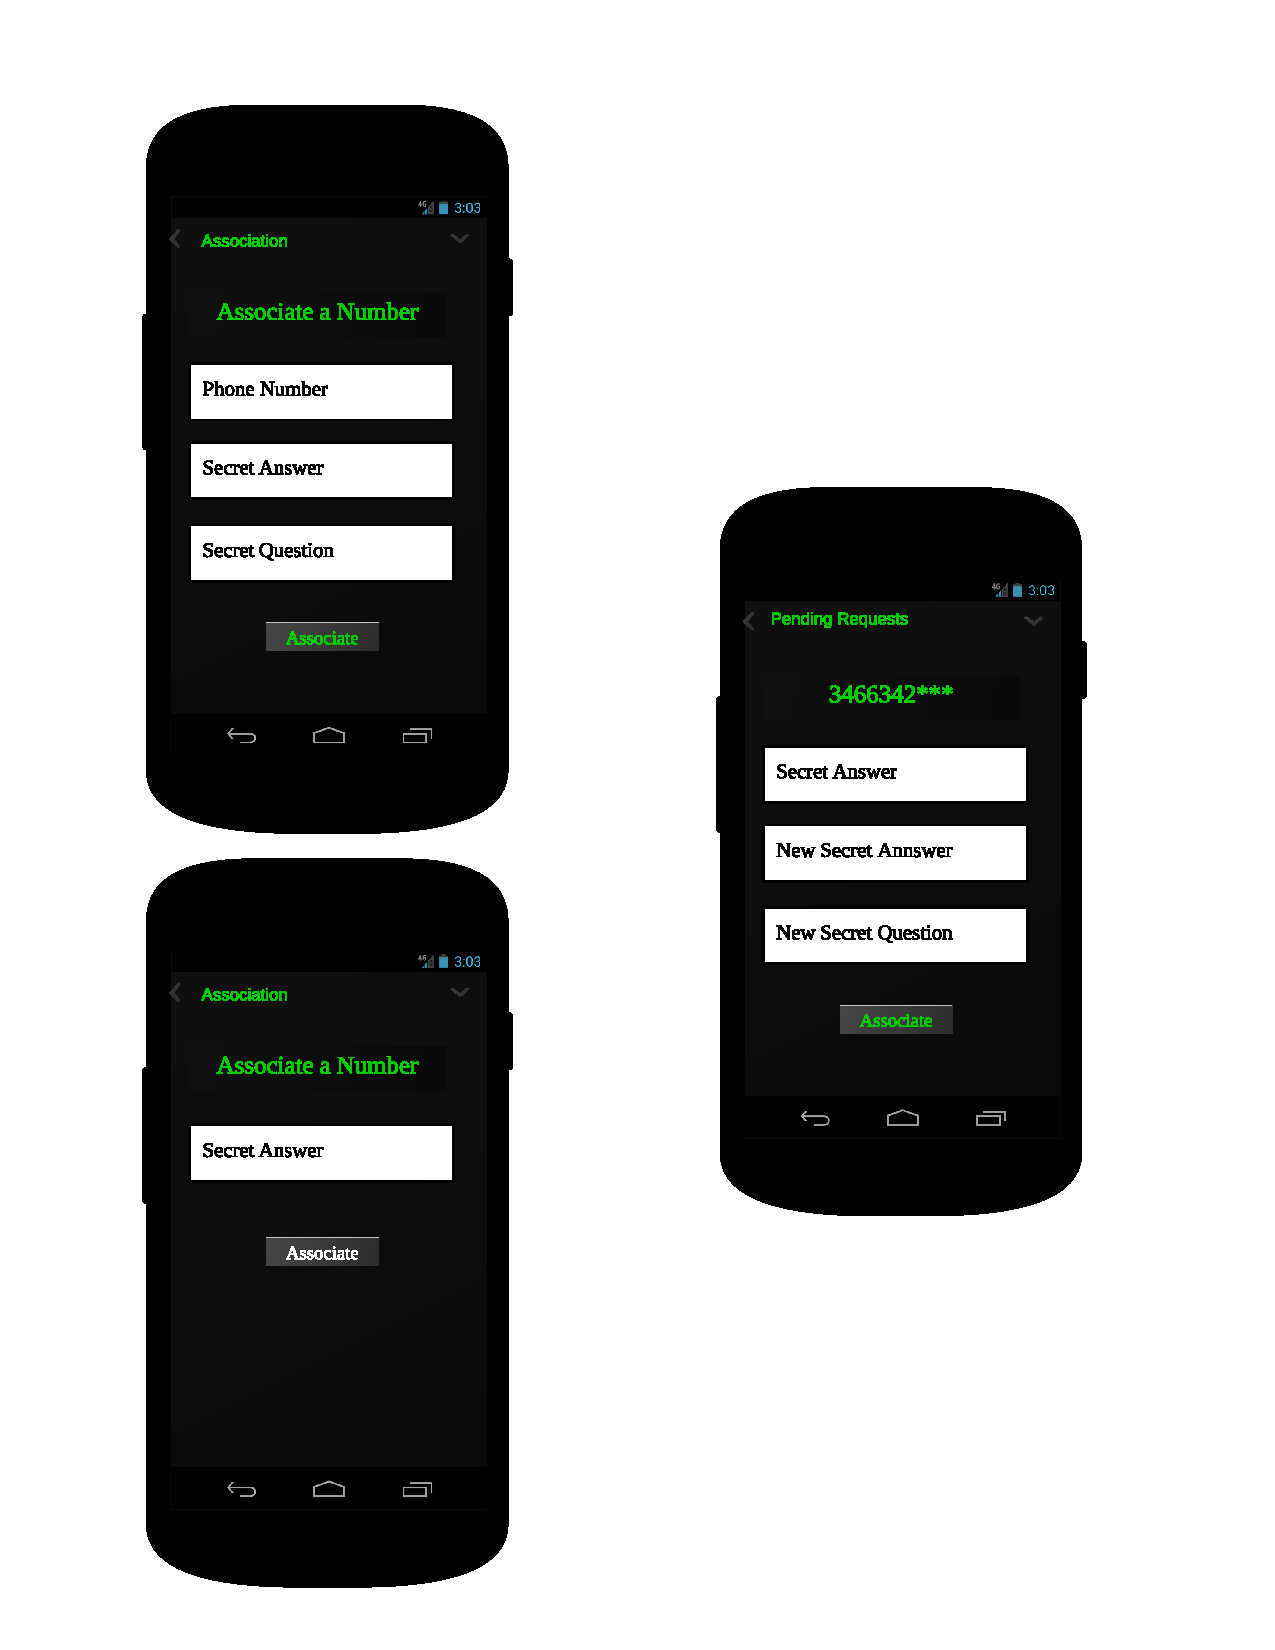
\includegraphics[scale=0.7]{images/SMP_design}

\section{Password Change}

The user types the old password, the new password and the confirmation new
password; the system checks whether the old one is correct and the new ones
are coherent and rules compliant (see initialization wizard use case). If not
an error message is prompted and nothing is done, otherwise the password is
succesfully updated and the user notified back.

\subsection{Activity Diagram}

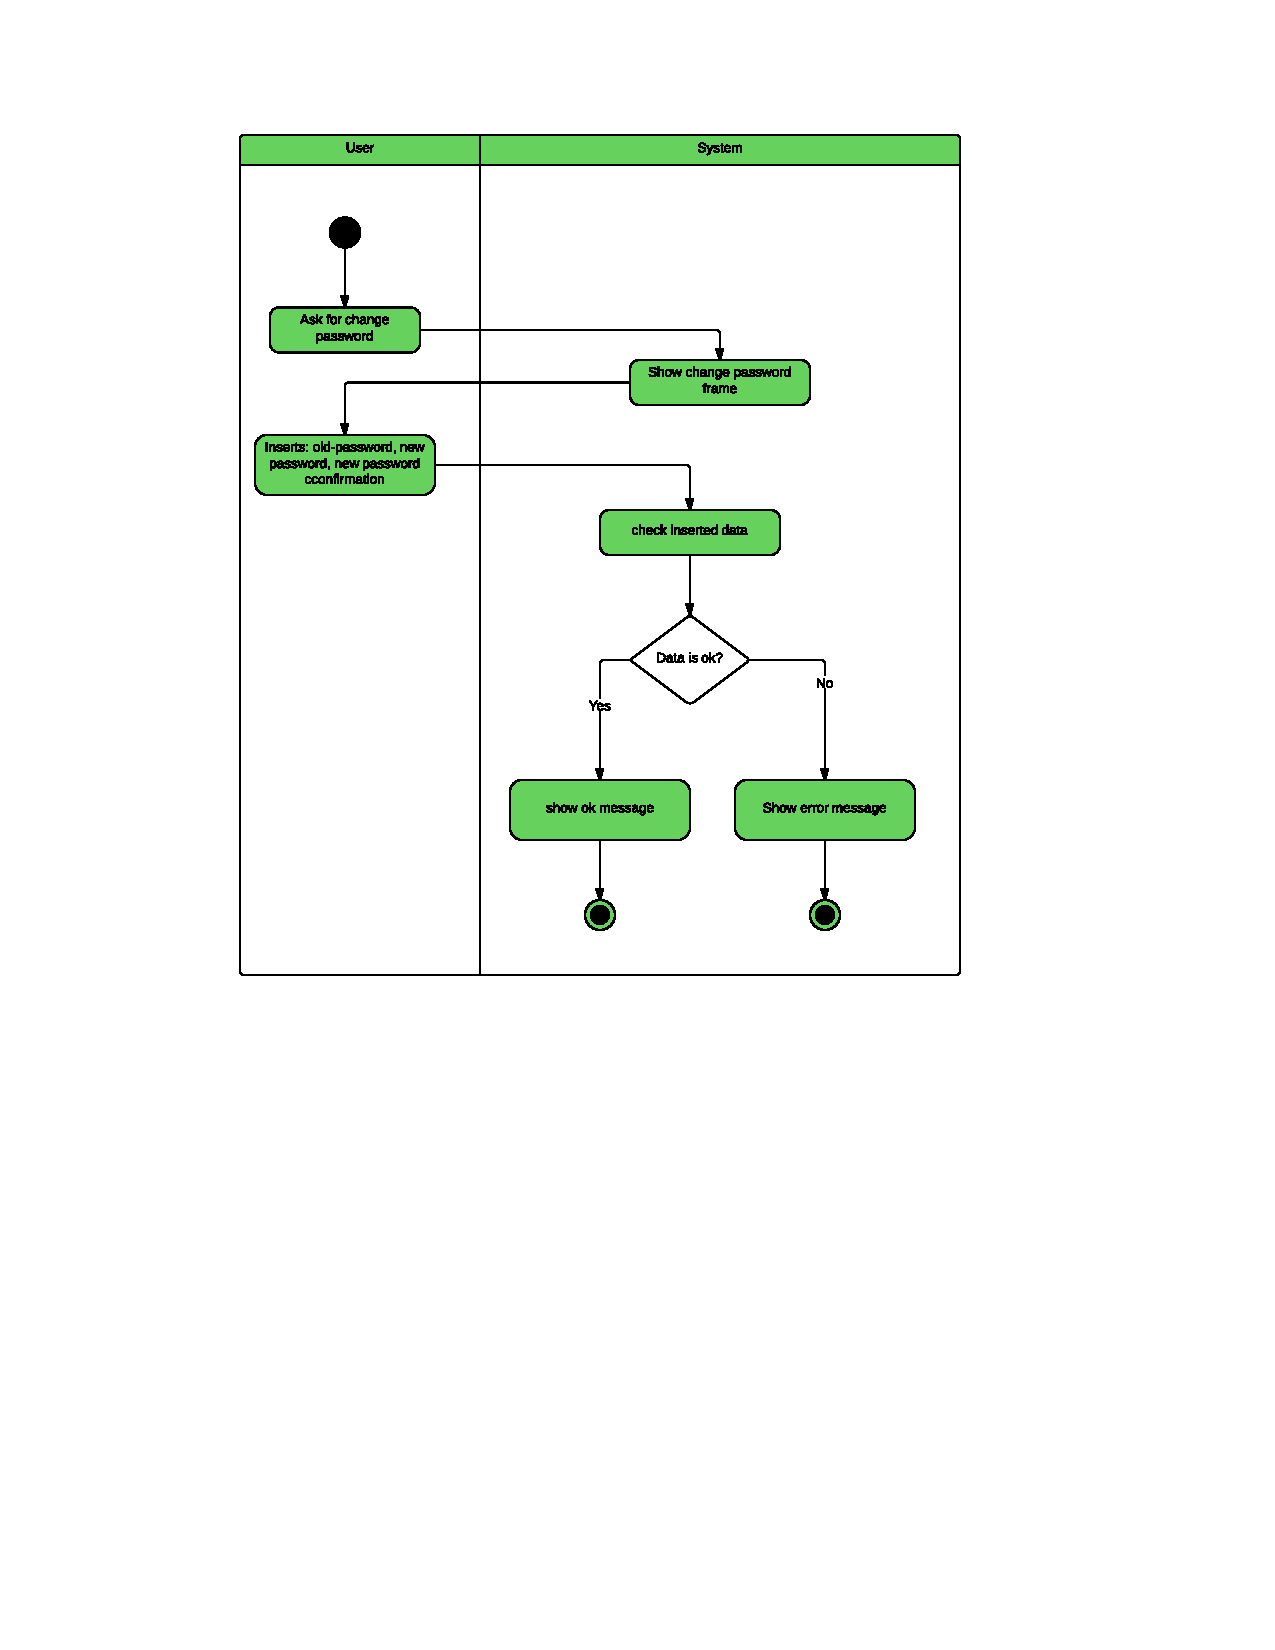
\includegraphics[scale=0.6]{images/ChangePassword_activity}

\newpage
\subsection{User Interface Design}

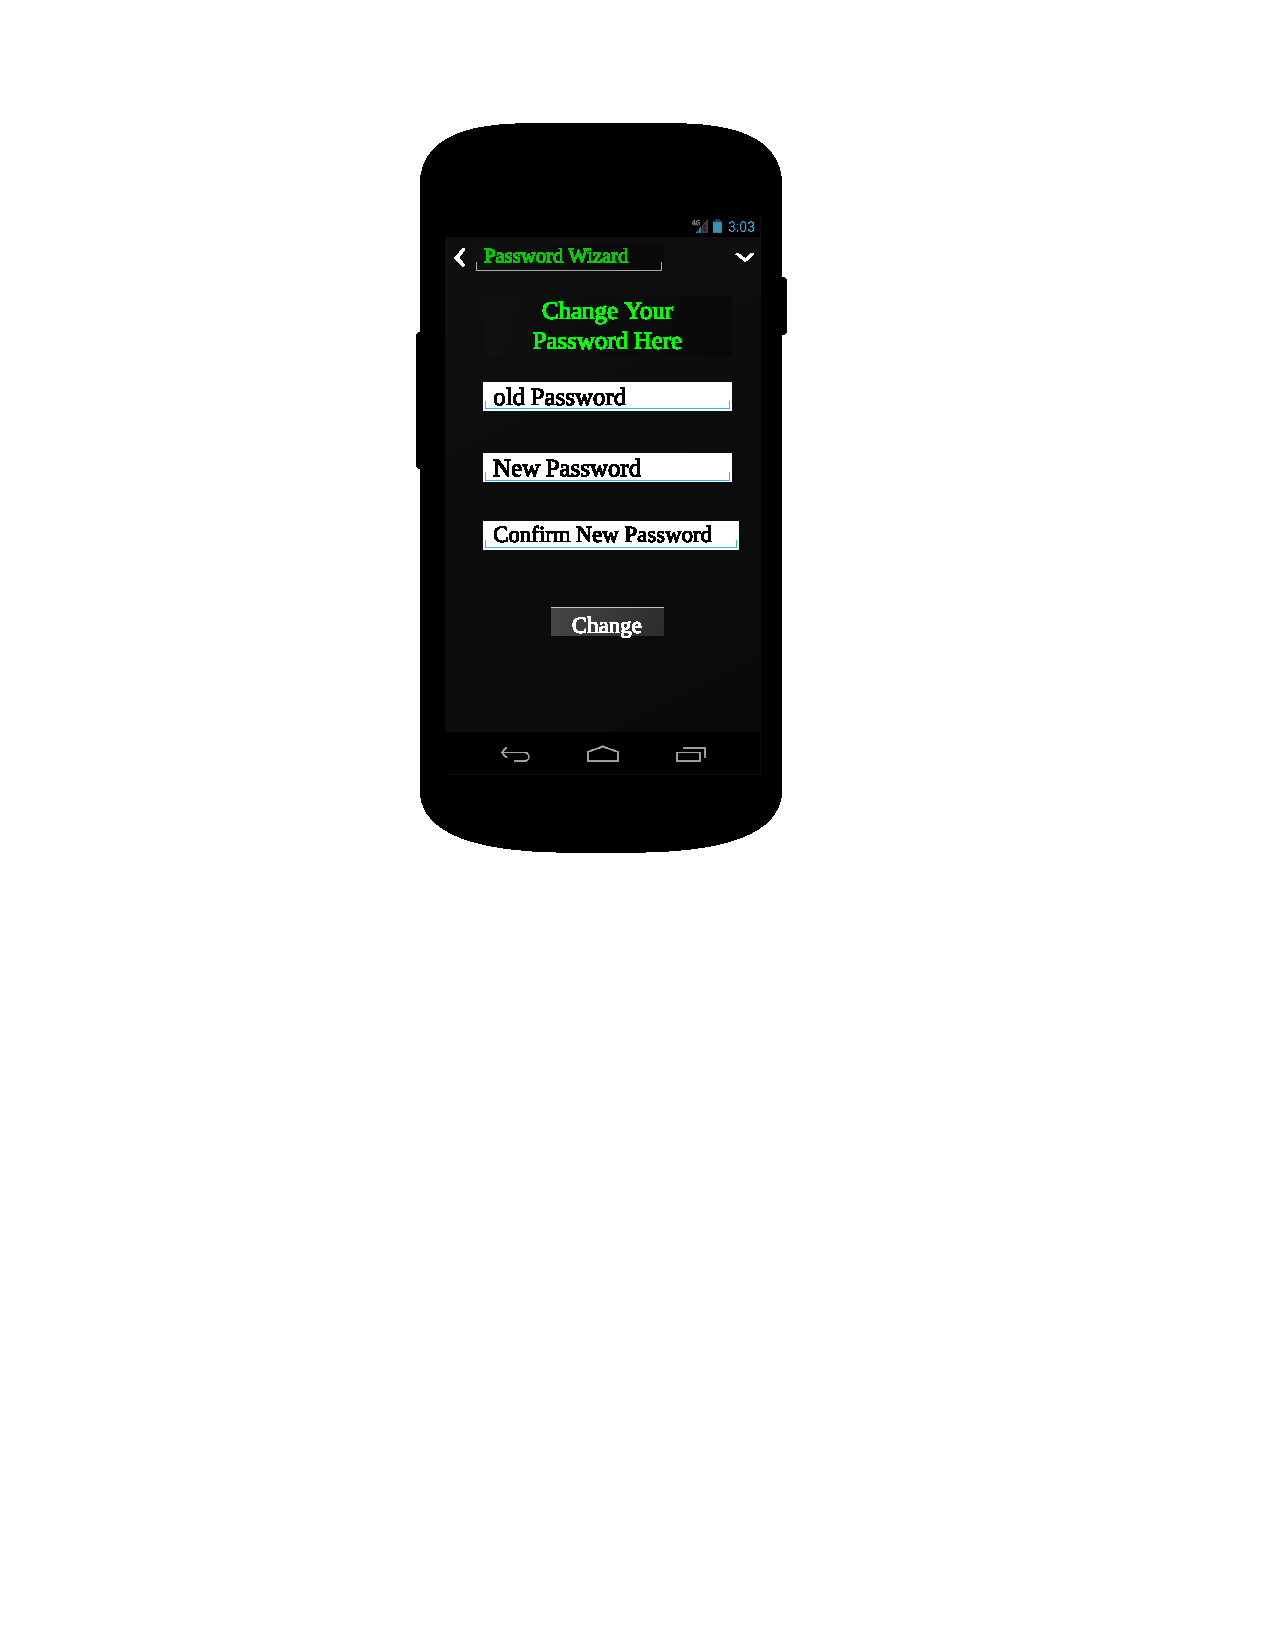
\includegraphics[scale=0.7]{images/PasswordChange_UI}

\section{Unilateral Deassociation}

The user selects from the list of his contacts the one he wants to deassociate
with and confirms his intention by clicking on the apposite button. The
relative preferences are deleted, but the "target" is not notified.


\newpage
\subsection{Activity Diagram}

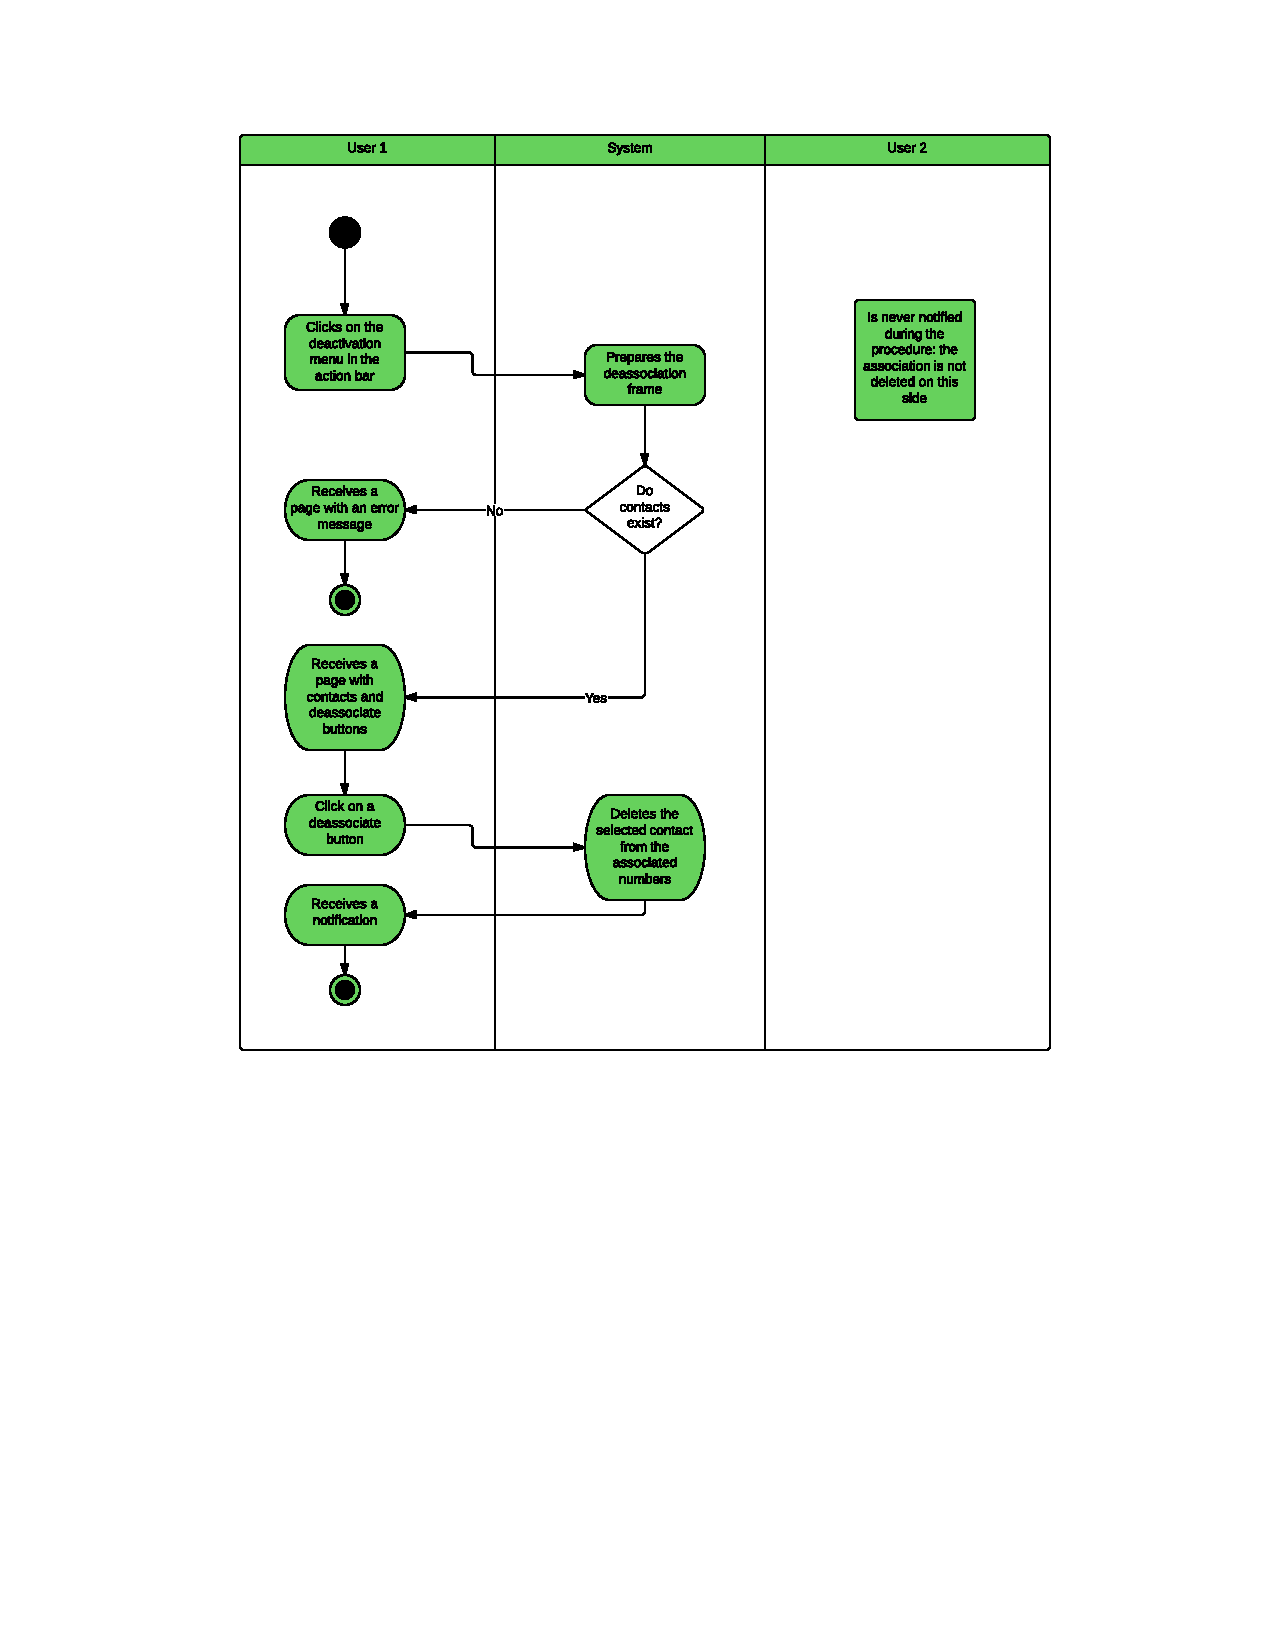
\includegraphics[scale=0.7]{images/UnilateralDeassociation}

\newpage
\subsection{User Interface Design}

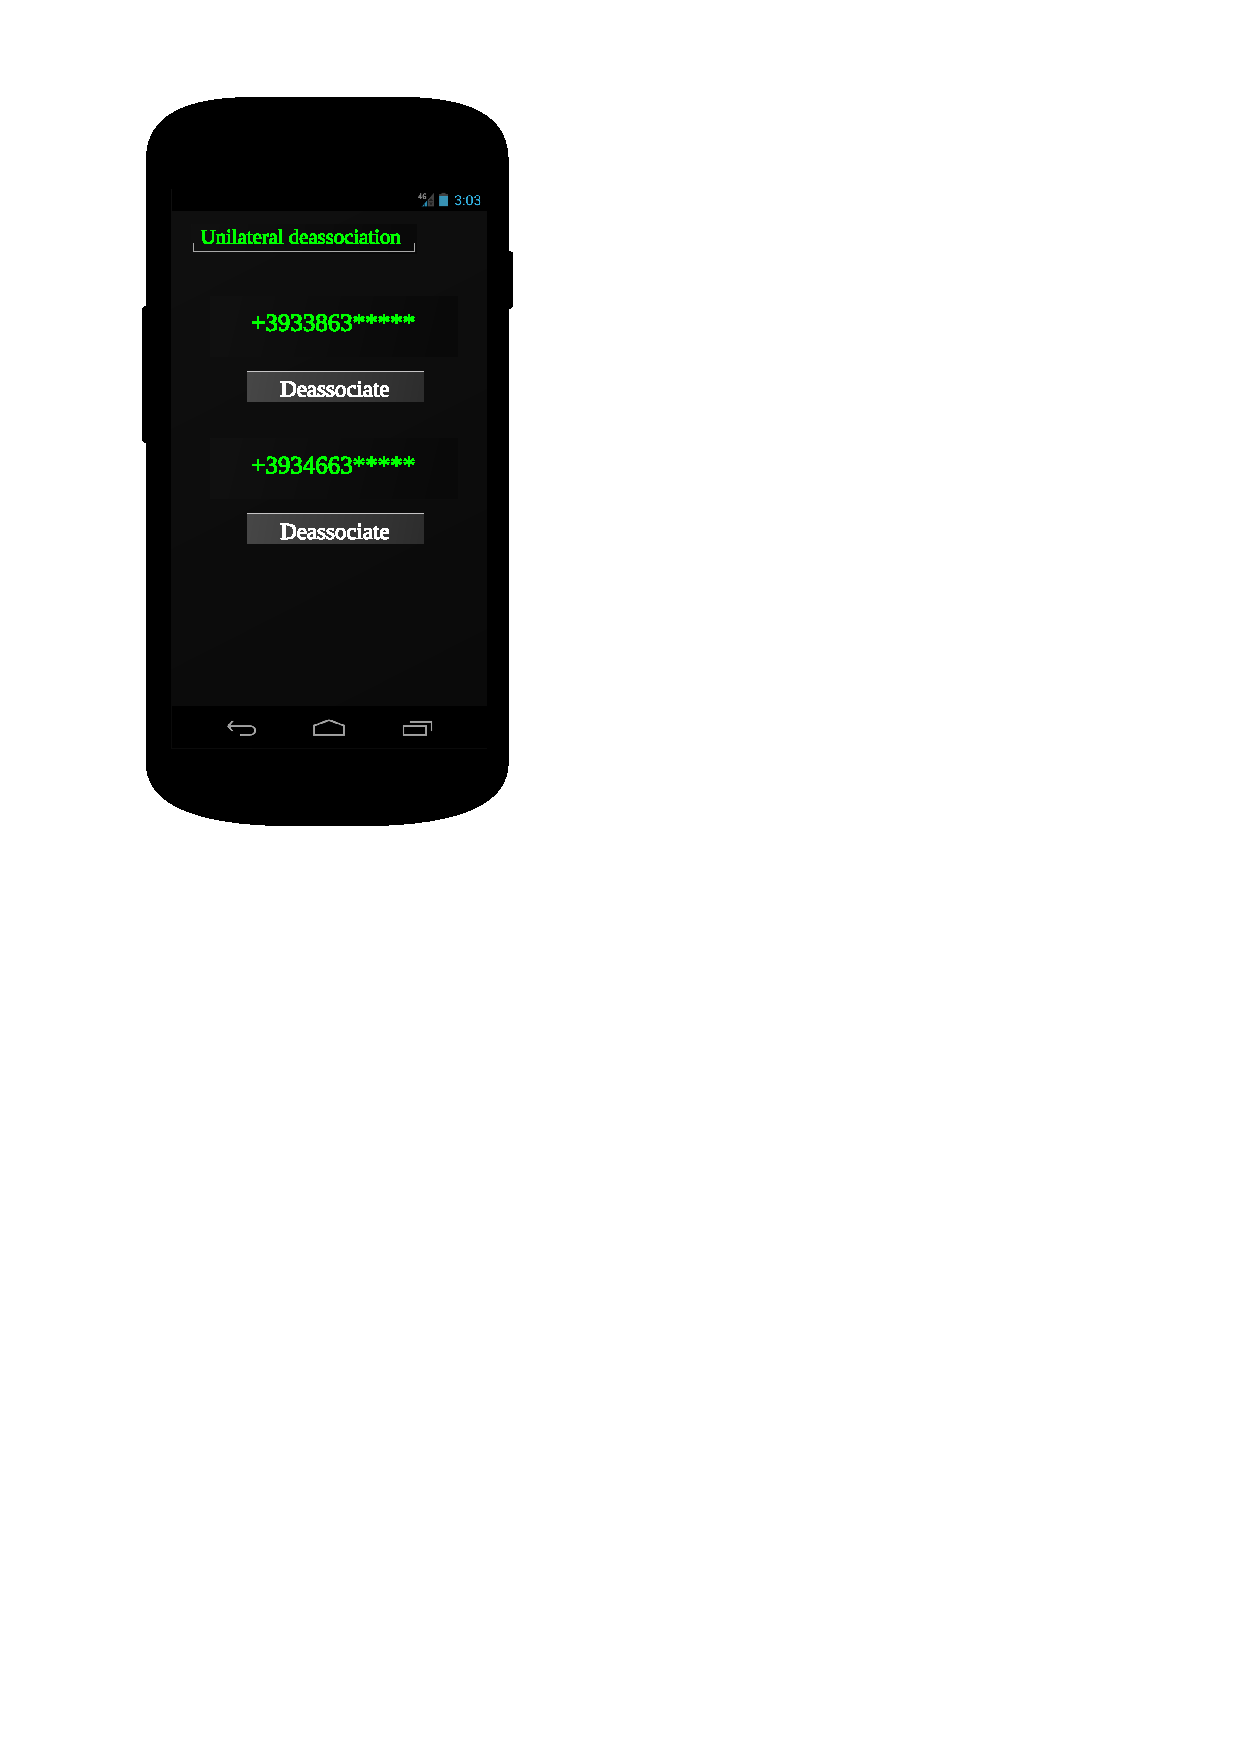
\includegraphics[scale=0.7]{images/DeassociationAndroid}

\section{Remote Localization}

The user (which sees a list of his contacts/associated numbers) types the
target password and confirms the intention to send a localize command by
clicking on the apposite button. After an handshake (done by sms exchanging)
the target phone executes the command and sends back a failure message or
his actual coordinates. The original sender receives a notification with a map
and a marker indicating the target position.


\newpage
\subsection{Activity Diagram}

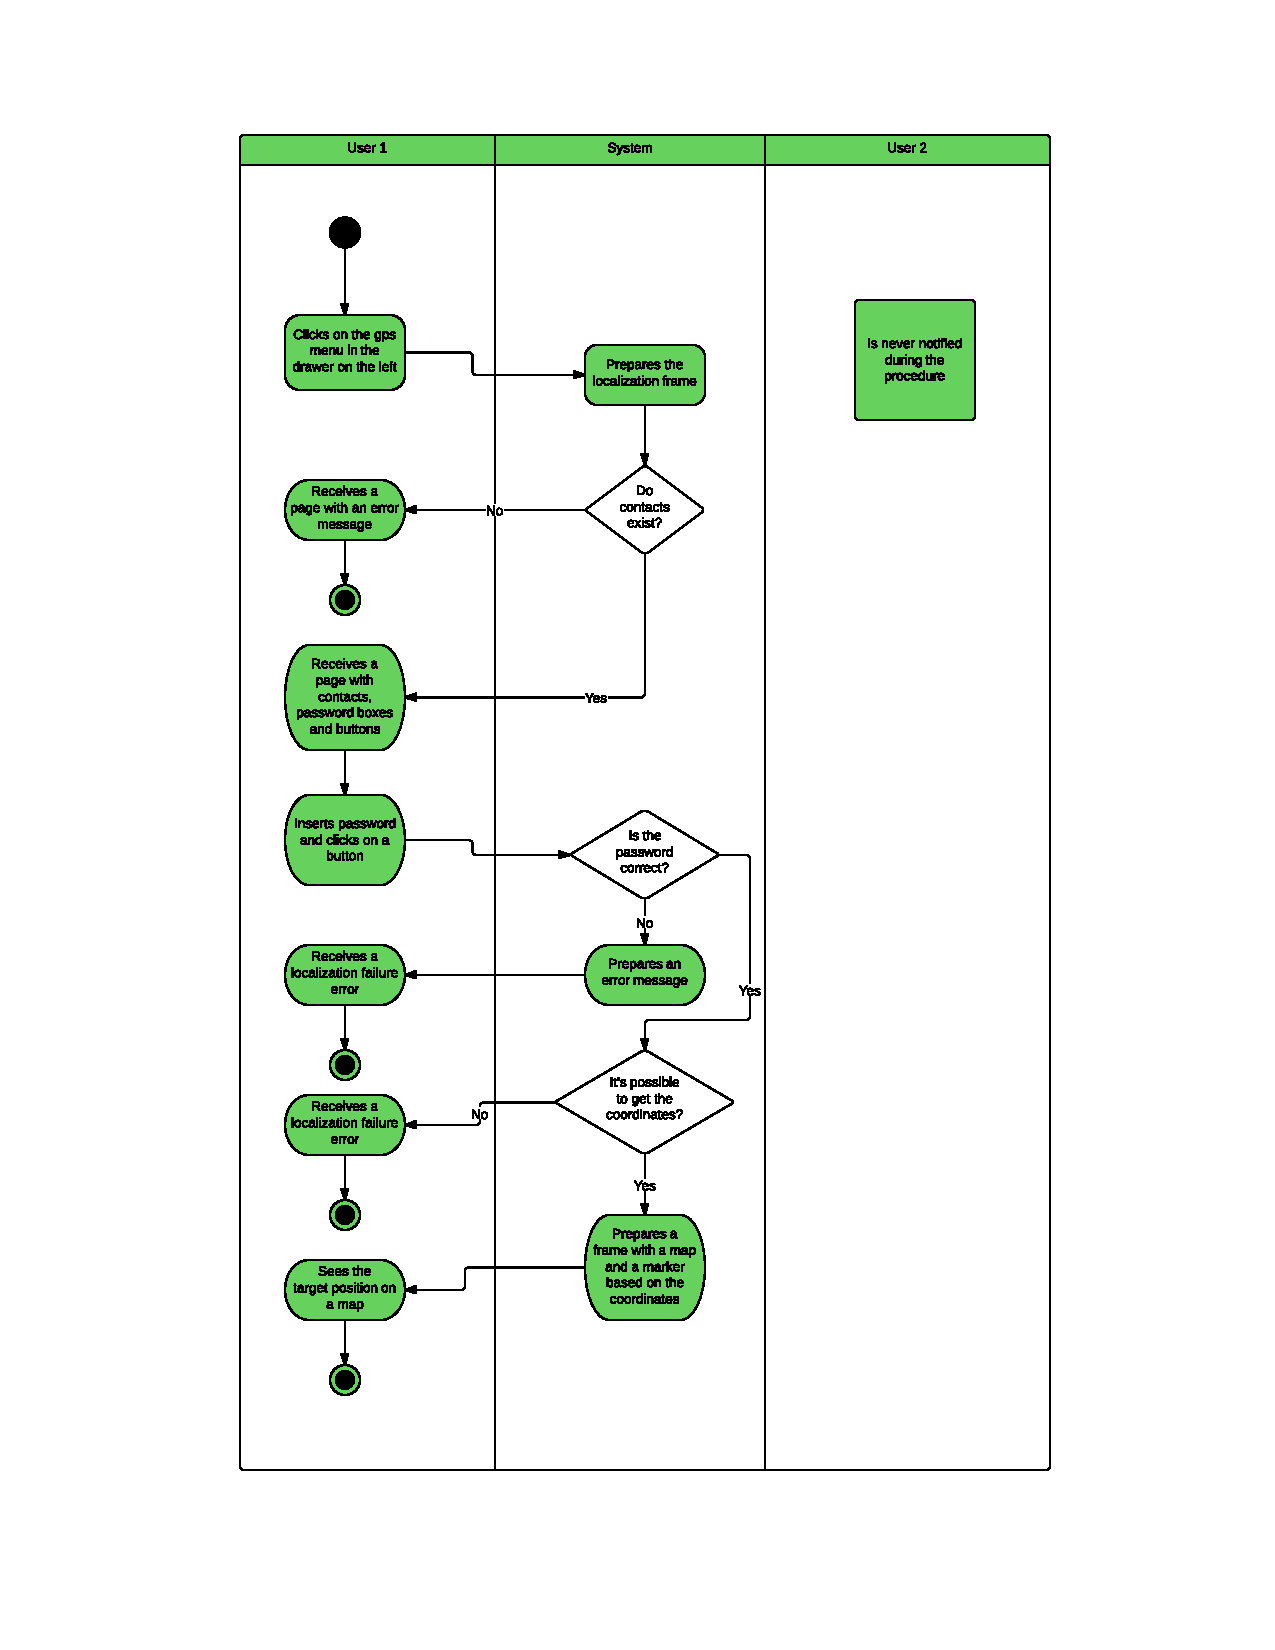
\includegraphics[scale=0.7]{images/Localization}

\newpage
\subsection{User Interface Design}

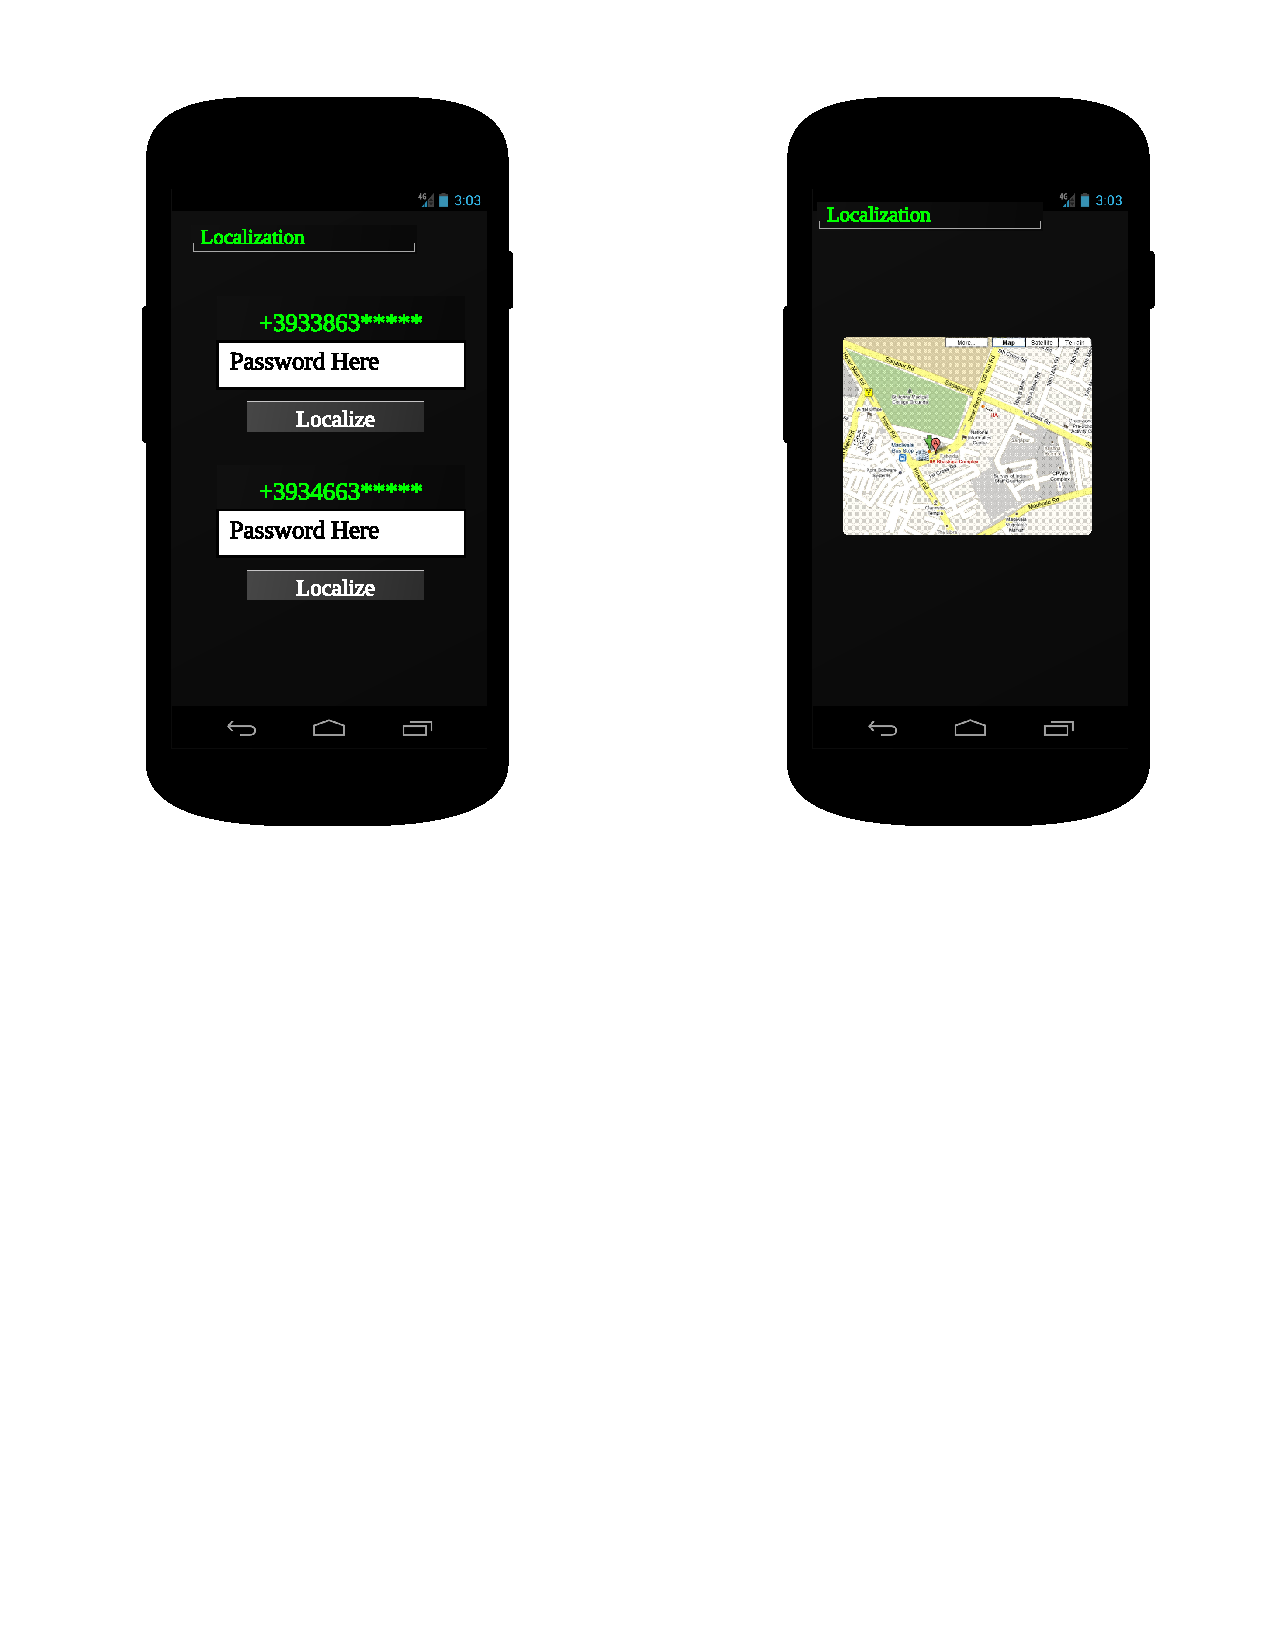
\includegraphics[scale=0.7]{images/Localization_mobile}

\section{Mobile Phone Mark}
The mark features have been left unimplemented: they are in the TODO list,
so no use cases for now.


\newpage
%\subsection{Activity Diagram}

%\newpage
%\subsection{User Interface Design}

\section{Remote Alarm Triggering: Activate and Deactivate Siren}

The user selects from his contacts the target and confirms by clicking on a
specific button the will to send a siren on/siren off command. The command
session is similar to the localization one: the only difference is that the re-
turned message is only an ack or a failure code. The siren off is simply ignored
if the alarm in not active. There is also a feature which allows a user to turn
off locally a siren by inserting the password and clicking on the button.

\newpage
\subsection{Activity Diagram}

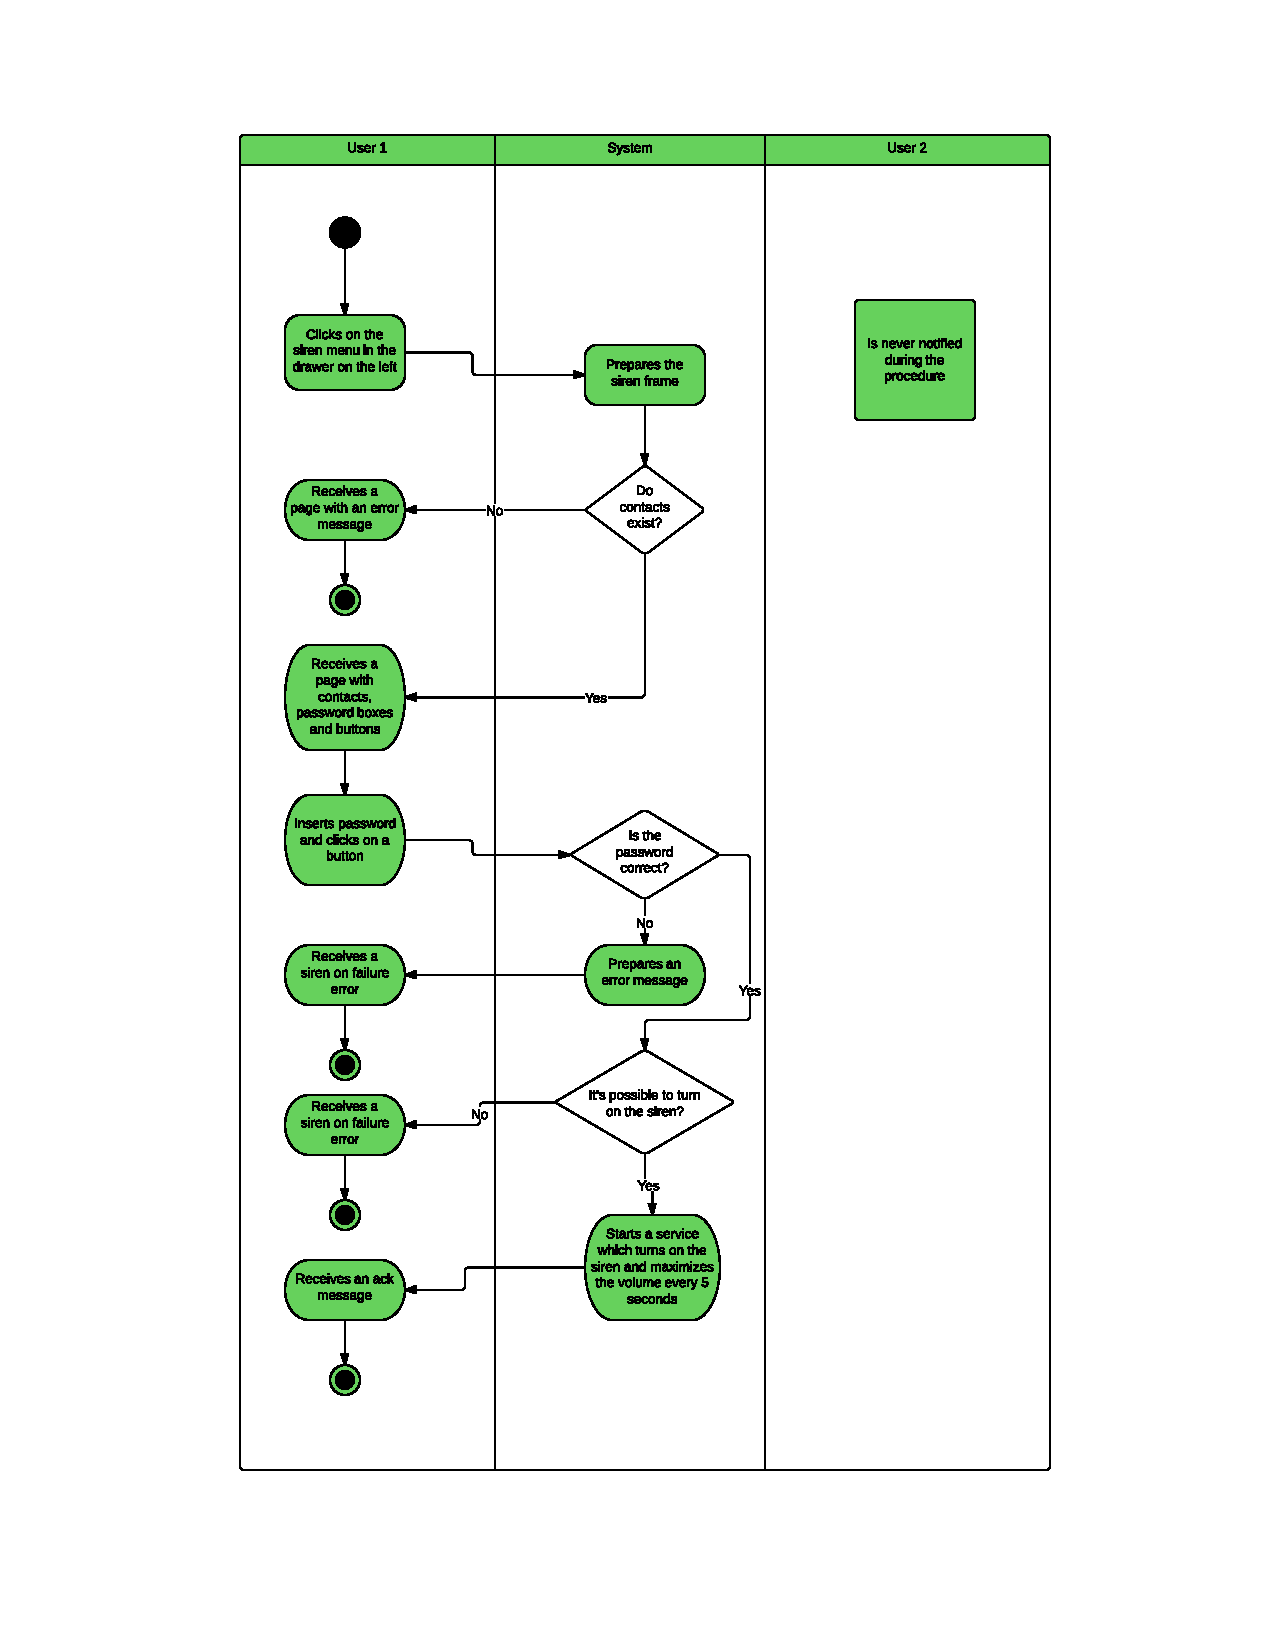
\includegraphics[scale=0.7]{images/SirenOn}
\newpage
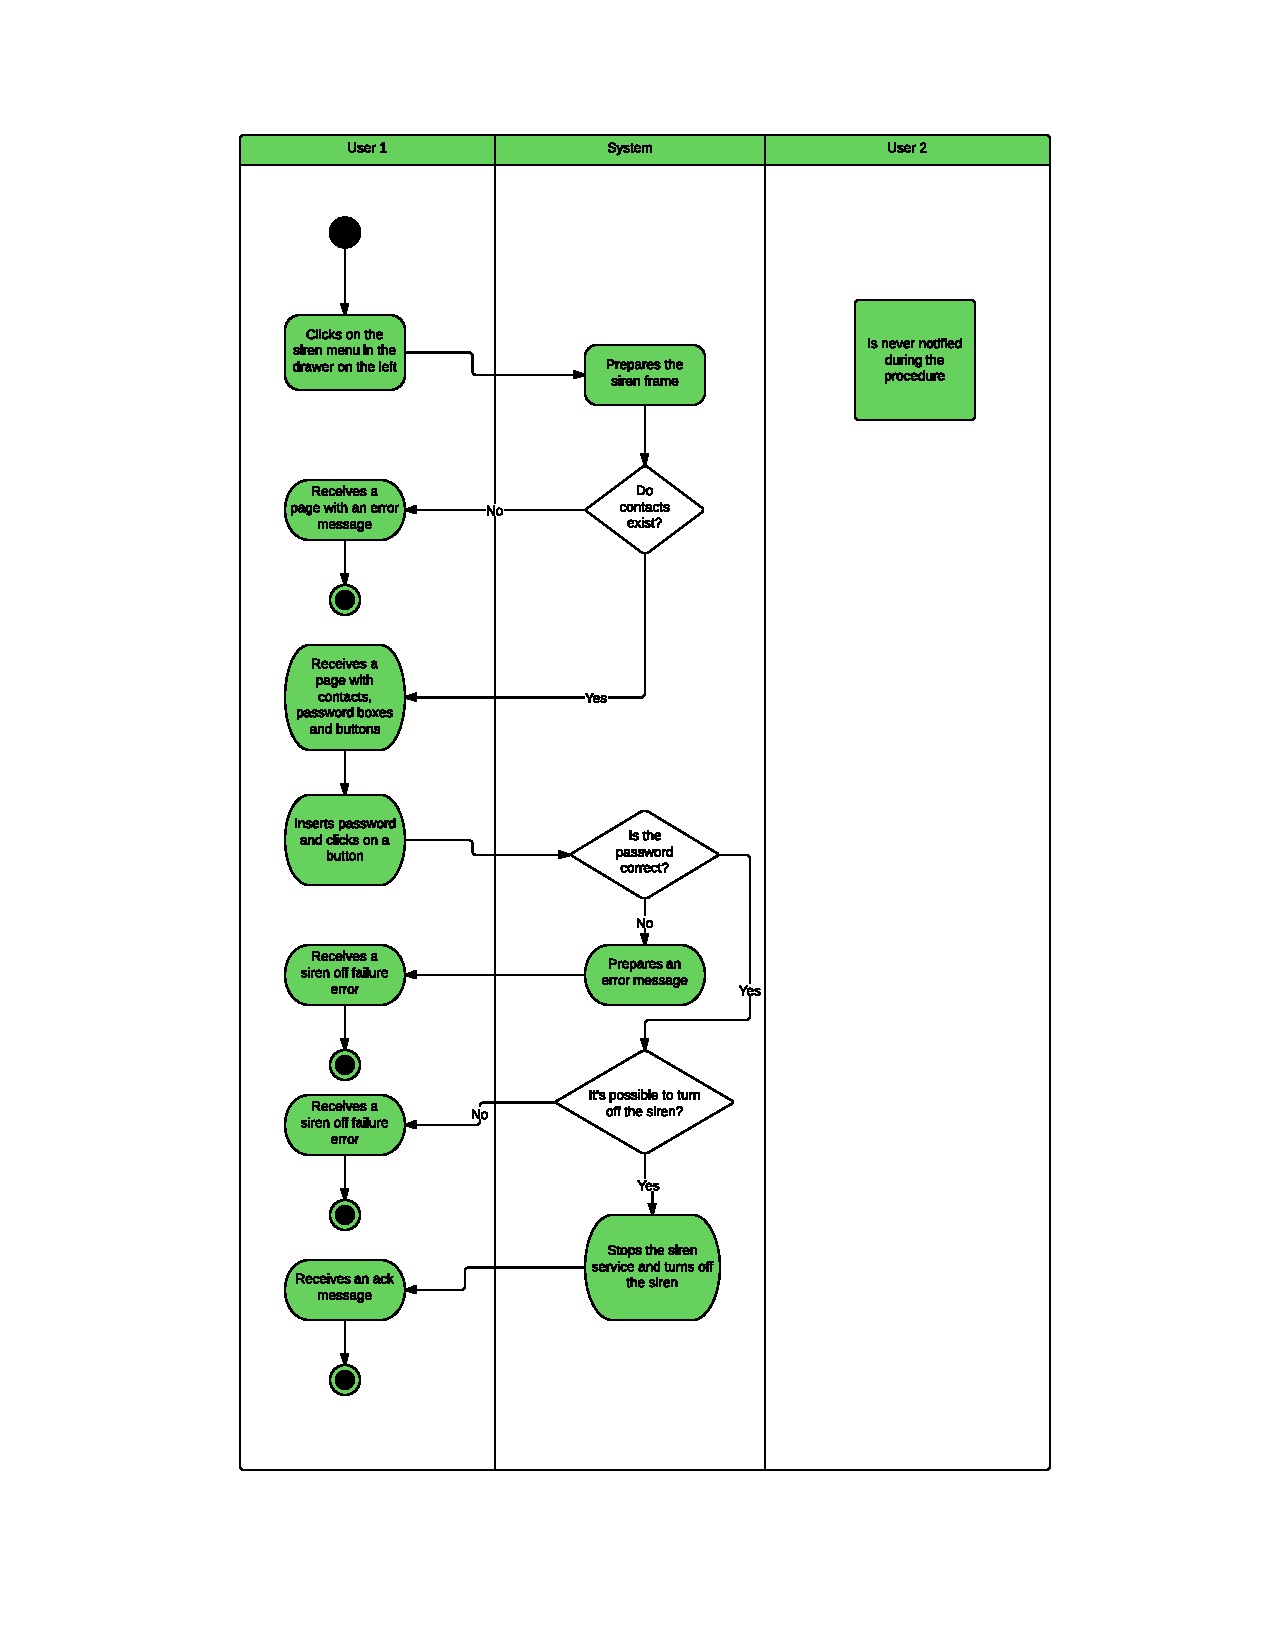
\includegraphics[scale=0.7]{images/SirenOff}
\newpage
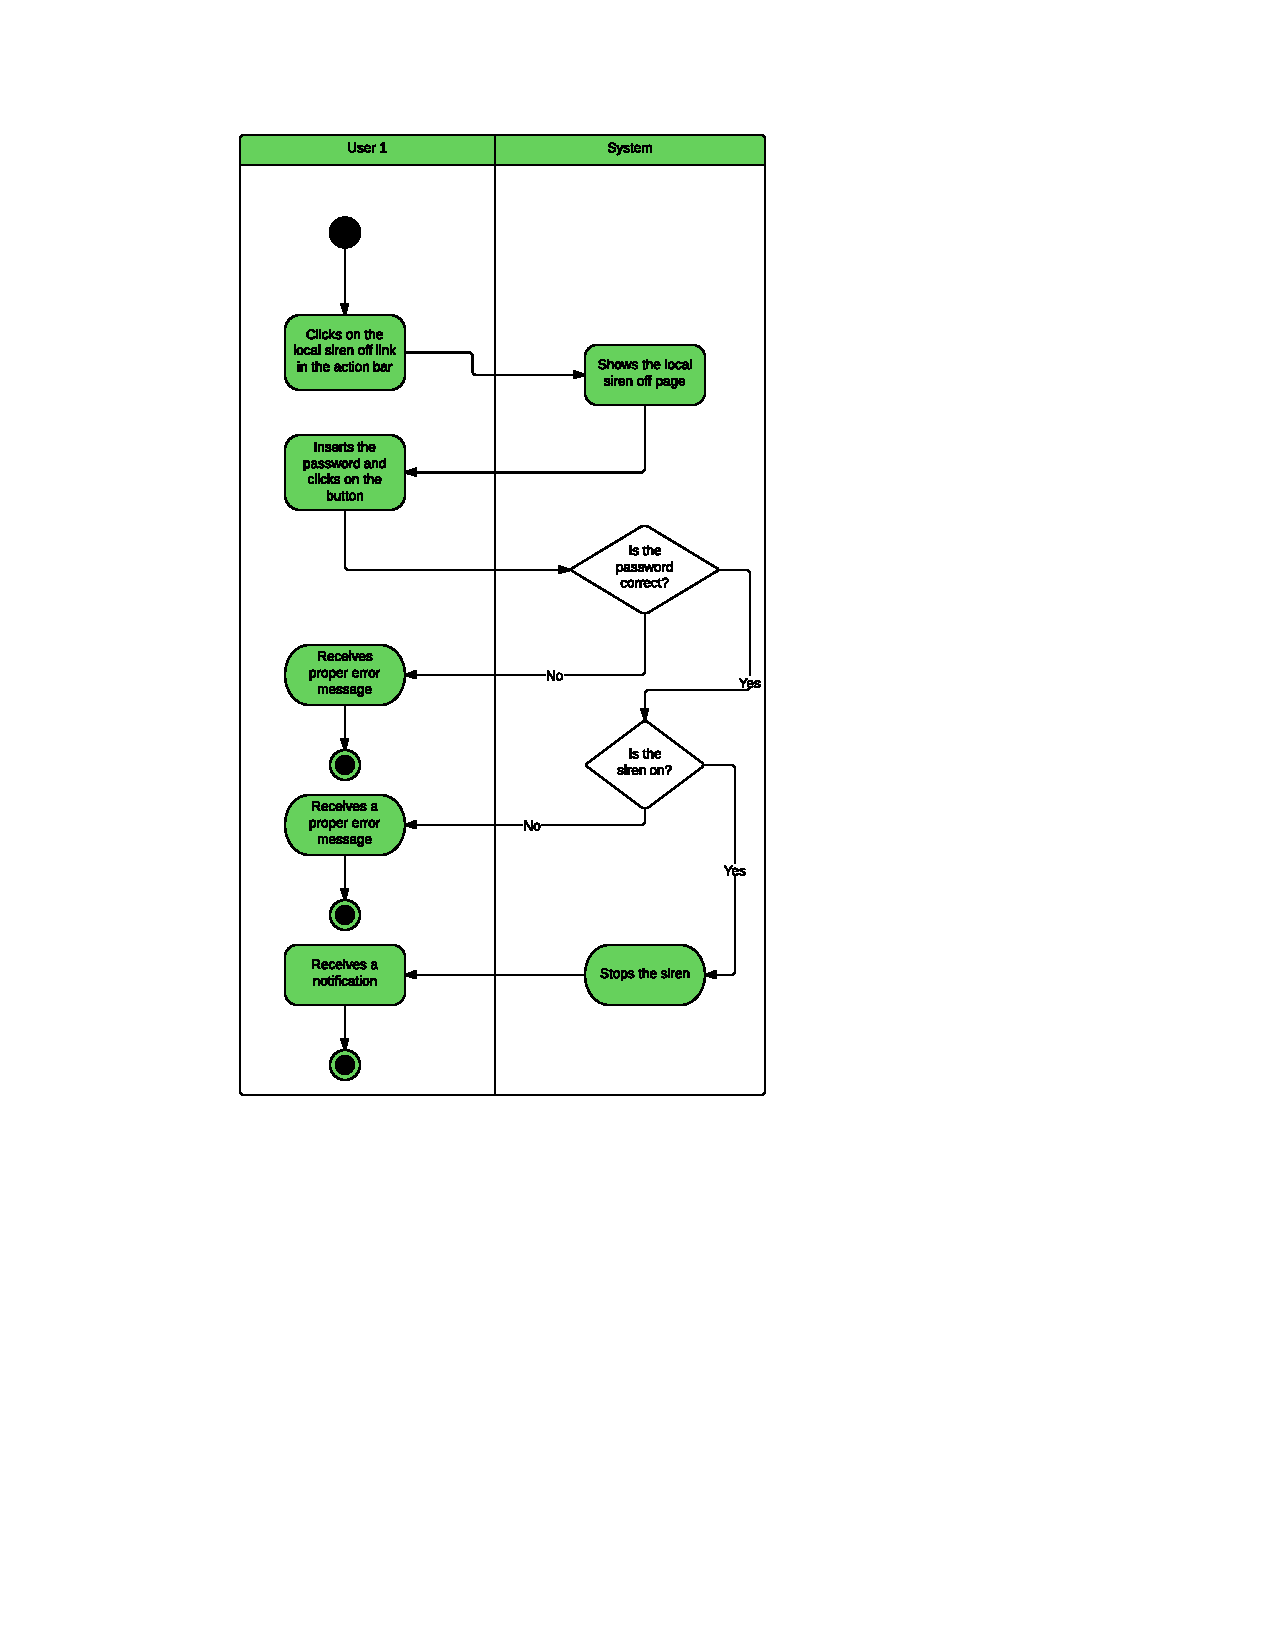
\includegraphics[scale=0.7]{images/localsirenoff}

\newpage
\subsection{User Interface Design}

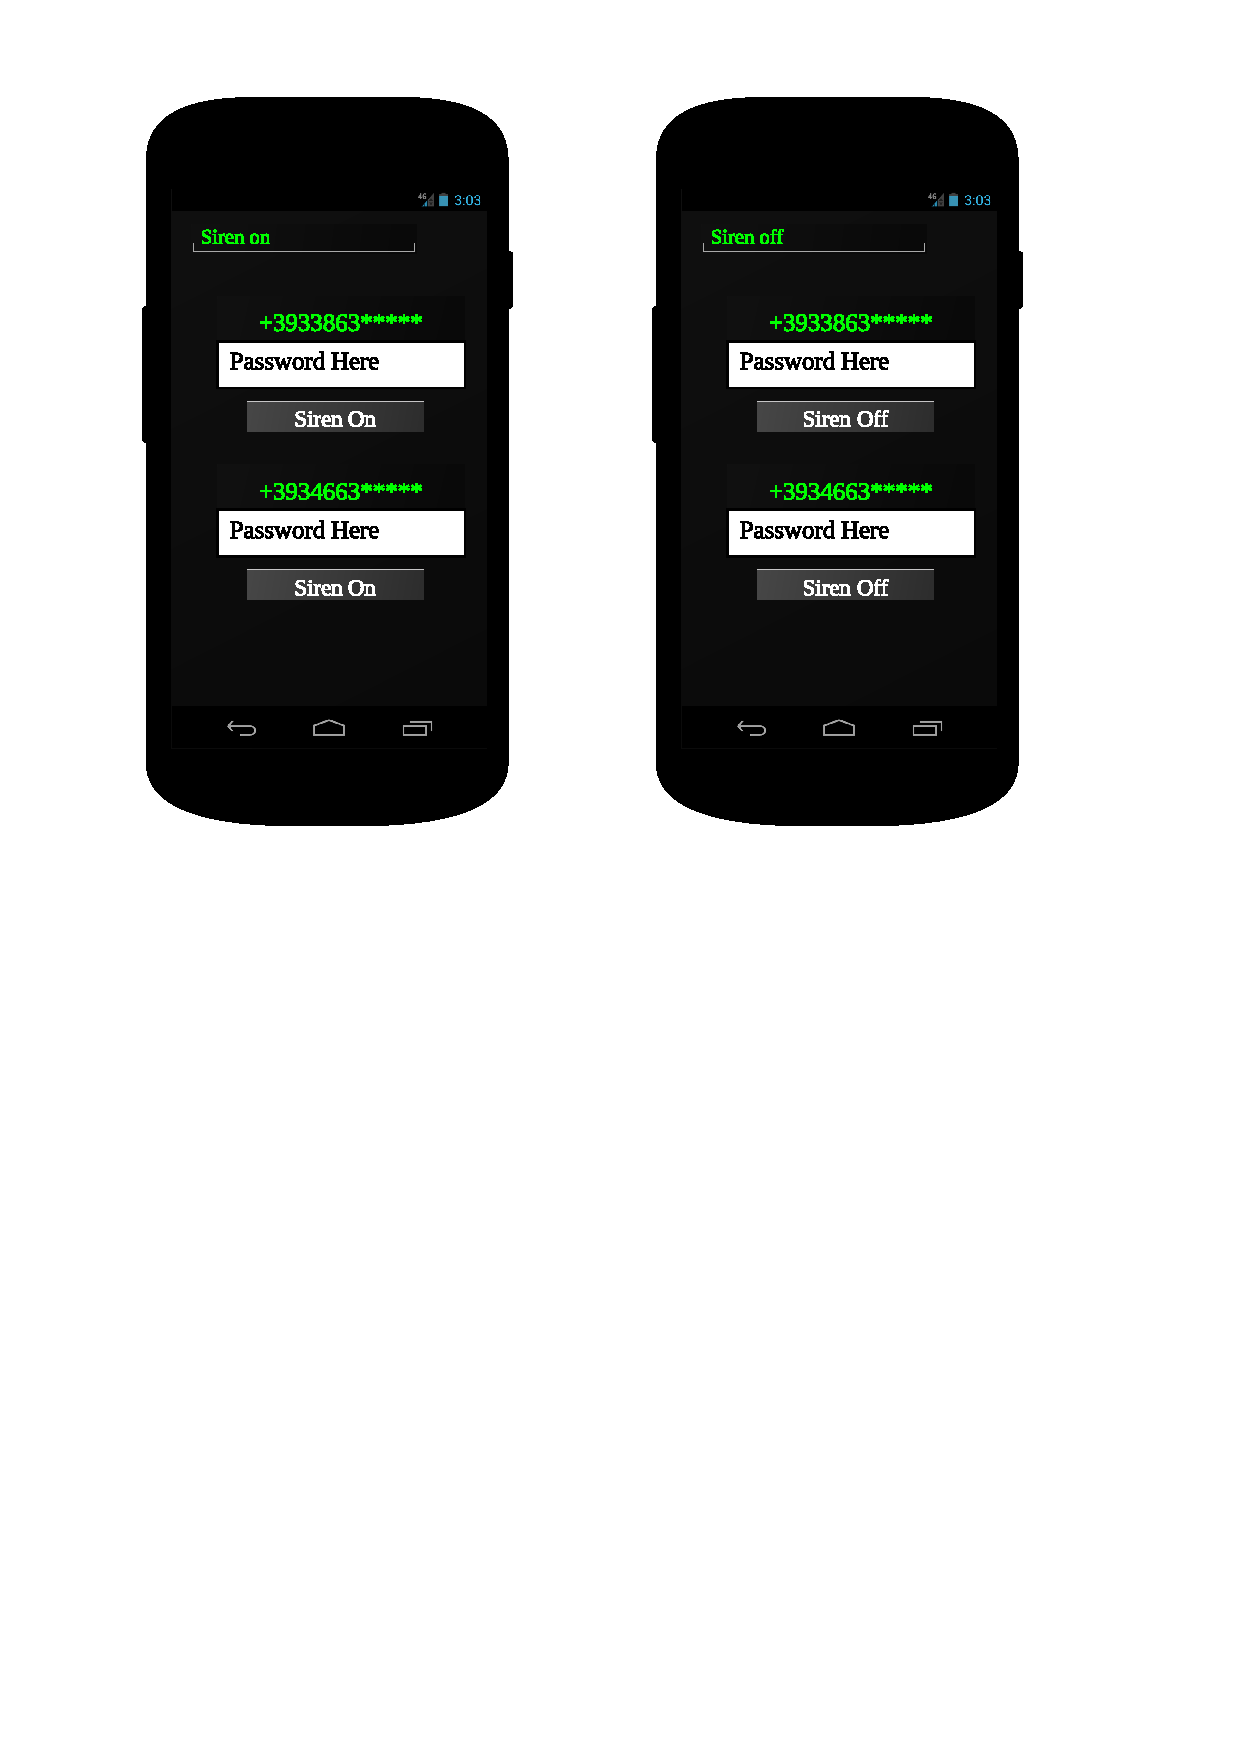
\includegraphics[scale=0.7]{images/sirenonoff_mobile}


\section{Perimeter Selection}

The perimeter selection feature, when activated, must select a circle area
centered where the cellphone is at that moment, and trigger an alarm if the
mobile phone exits from there. The circular limit has also to be visible on a
map on the telephone.


\newpage
\subsection{Activity Diagram}

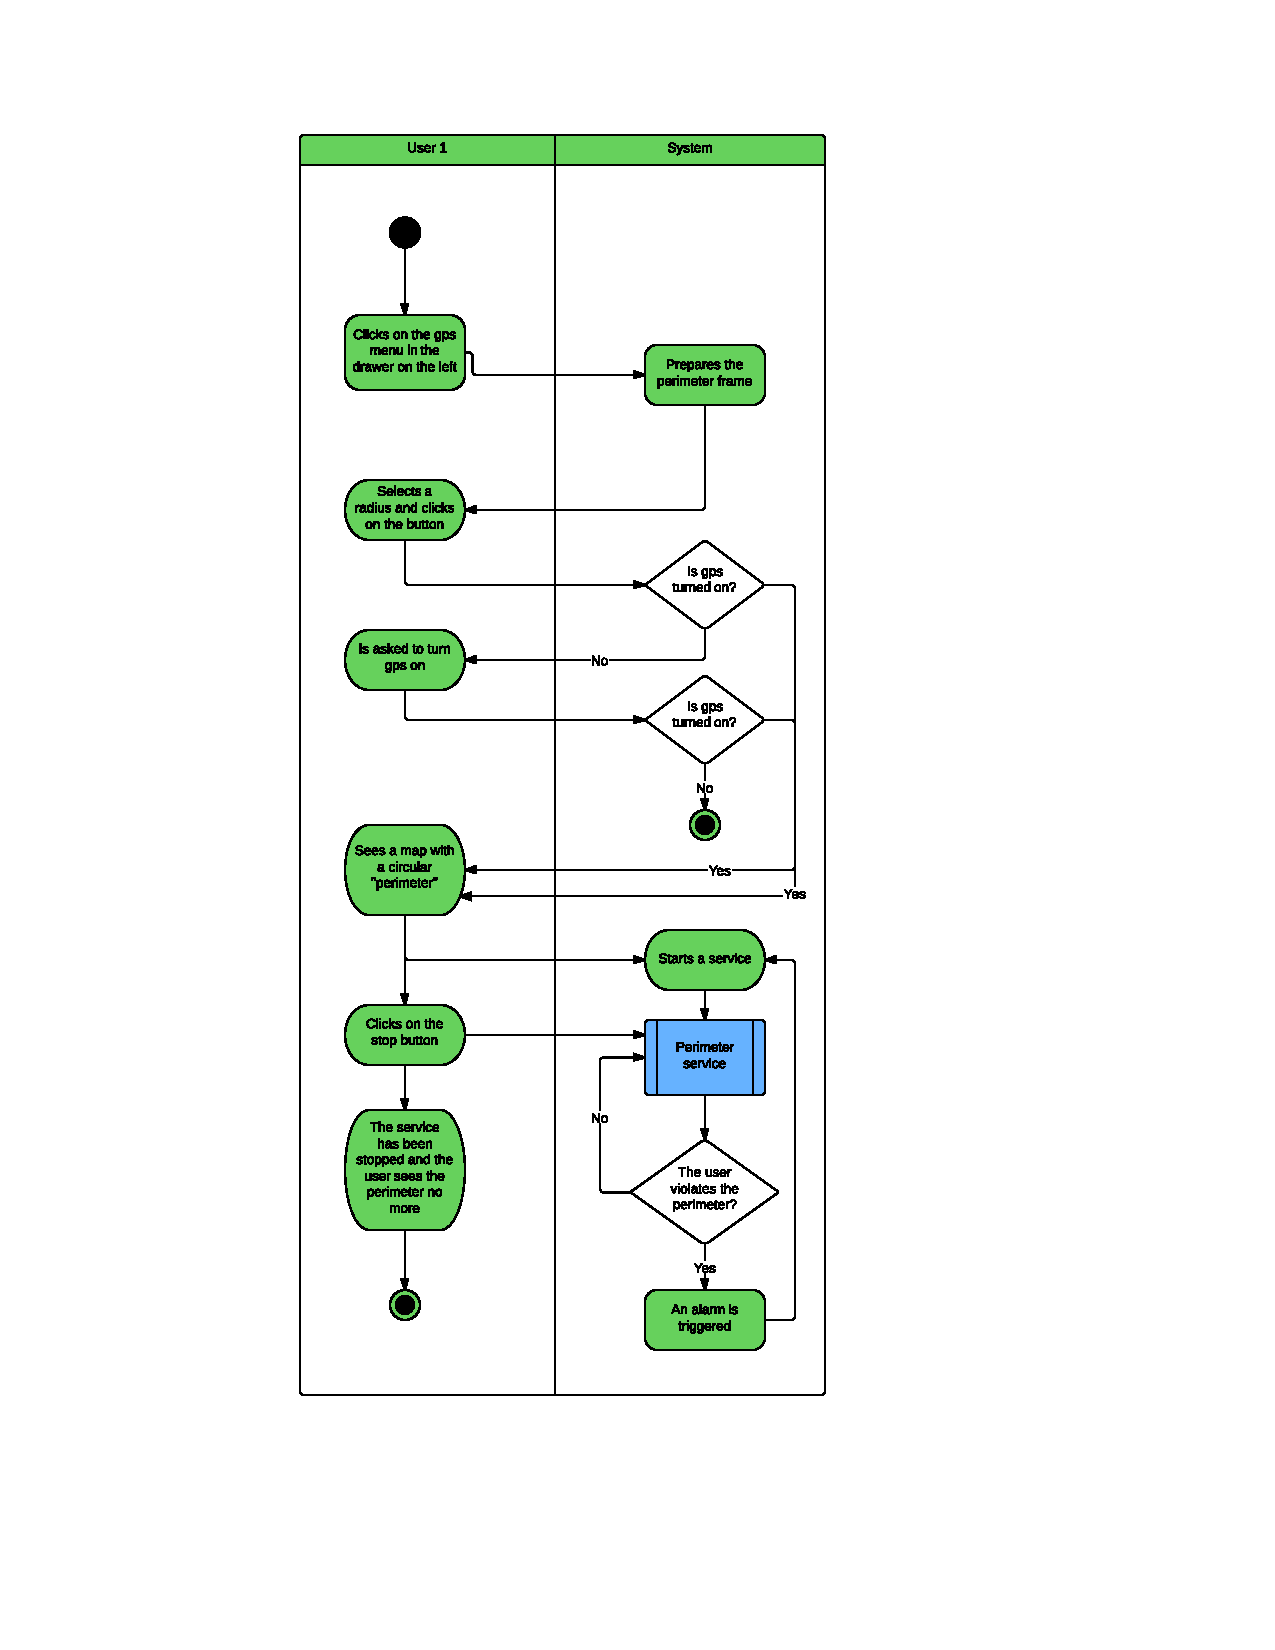
\includegraphics[scale=0.7]{images/Perimeter}

\newpage
\subsection{User Interface Design}

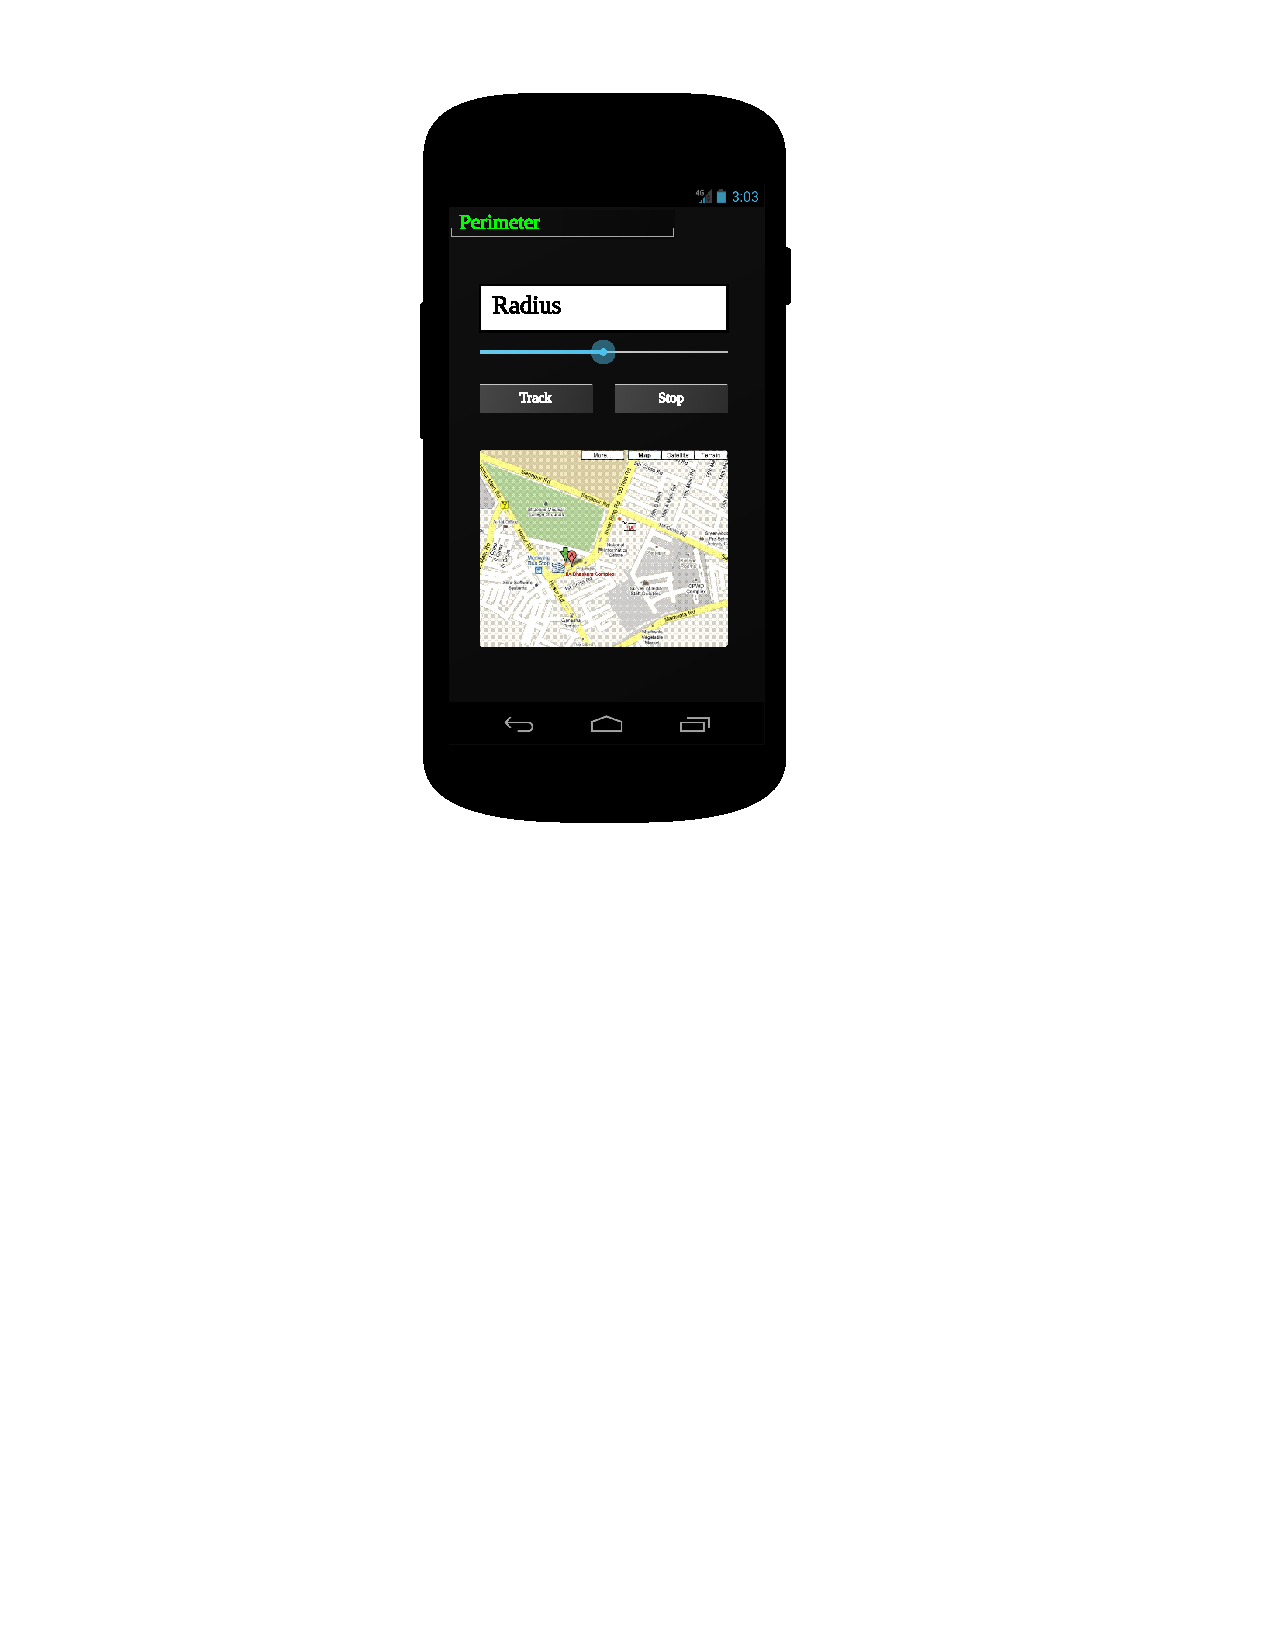
\includegraphics[scale=0.7]{images/Perimeter_mobile}

%\include{contents/StateDynamicsViewpoint}
%\include{contents/InteractionViewpoint}
% Appendici


% --------------------------------------------------------------------------------------------------------------------
% Bibliografia - nothing for now!
%\bibliographystyle{plain}
%\input{contents/bibliography.tex}

% --------------------------------------------------------------------------------------------------------------------

\end{document}